\chapter{Machine background from the Beam Delivery and Final-Focus systems}

\begin{chapterabstract}
 Particles produced in beam interactions with the accelerator components present another source of background for particle detectors.
 With thorough simulations and measurements,  the characteristics of the machine background can be understood, and its effect on the detector performances evaluated.
 \\In the first part of this chapter, shielding options against muons that are created in the Beam Delivery System of the International Linear Collider are discussed.
 The simulation of the muon production was done with \mucarlo, before the occupancy in the Silicon Detector was investigated in a full detector simulation.
 \\The second part of this chapter describes measurements of the machine background done at the Accelerator Test Facility 2.
 These measurements are then compared to a simulation of ATF2 with the accelerator simulation framework \bdsim.
\end{chapterabstract}

\section{Muon background from the Beam Delivery System}
\label{BDS_Muons}
After the beam acceleration in the main linacs of the ILC, the Beam Delivery System (BDS) is the part of the accelerator that prepares the beams for collision.
As described in Section~\ref{ILC:layout:details}, it contains numerous subsystems and components for beam collimation and focusing. 
Depending on the aperture of the collimators, some fraction of the beam halo hits the collimator material, which has the desired effect of collimating the beam, but also the undesired effect of producing background particles.
\\For defining the beam halo, which surrounds the beam core, the beam core itself has to be defined first in terms of $\sigma_x$ and $\sigma_y$, which are the RMS beam size values at the beginning of the first collimator location in the BDS: $\sigma_x = $ \SI{146}{\micro\meter} and $\sigma_y = $ \SI{9}{\micro\meter}~\cite{Lewis}.
In this study, the core is defined as an ellipse with a horizontal size of $\pm 5\sigma_x$ and a vertical size of $\pm 36\sigma_y$ at the beginning of the BDS.
The beam halo is the elliptical ring around the beam core, covering 5-13$\sigma_x$ and 36-93$\sigma_y$.
The beam particle intensity in the core follows a $\frac{1}{r}$ distribution, and the beam power of the halo is normalized to \SI{0.1}{\percent} of the nominal beam power~\cite{Glens_muon_talk}.
\\From interactions between the beam halo and the material of the collimators along the beam line, muons are produced predominantly via the Bethe-Heitler process (see Figure~\ref{fig:BDS_Muons:Muon_production} (a)).
Beamstrahlung photons interact with the nuclei of the machine component material, and pair-produce muons.
A production contribution on a few percent level comes additionally from direct annihilation of positrons with atomic electrons~\cite{MuonBkg_1TeV}.
The Feynman diagram for the annihilation process is shown in Figure~\ref{fig:BDS_Muons:Muon_production} (b).
The muons are boosted in the beam direction, and are traveling towards the interaction region.\\
\begin{wrapfigure}{r}{0.4\textwidth}
    \centering
    \begin{subfigure}[b]{0.4\textwidth}\centering
    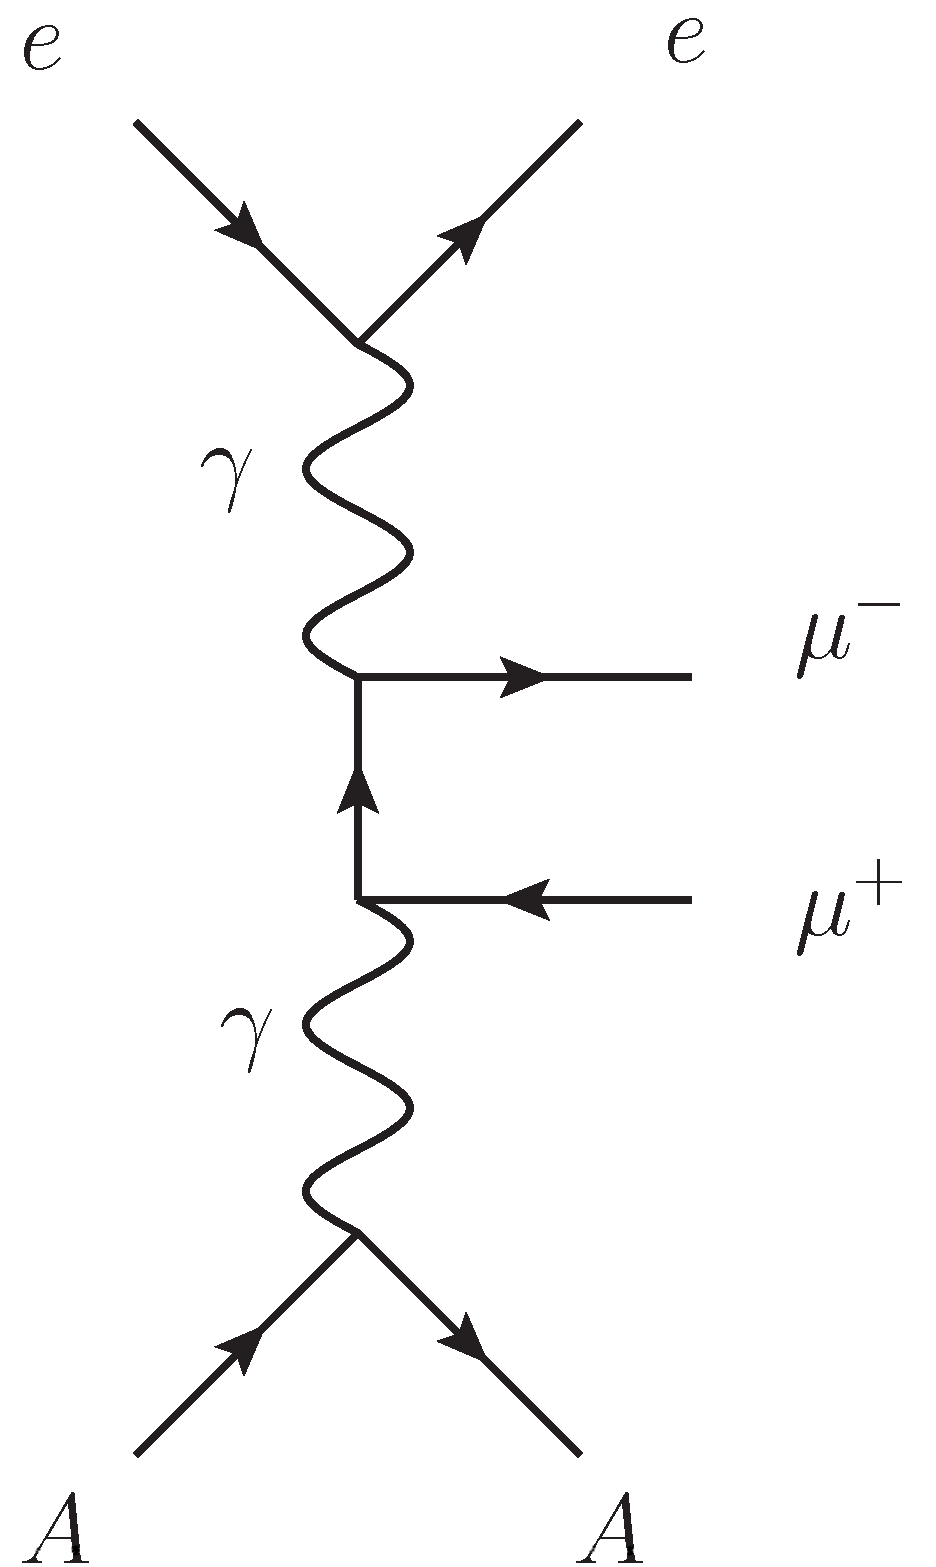
\includegraphics[width=0.5\textwidth]{Feynman_diagrams/Jaxo_BetheHeitler.png}
    \caption{Bethe-Heitler}
    \end{subfigure}\\
    \begin{subfigure}[b]{0.4\textwidth}\centering
    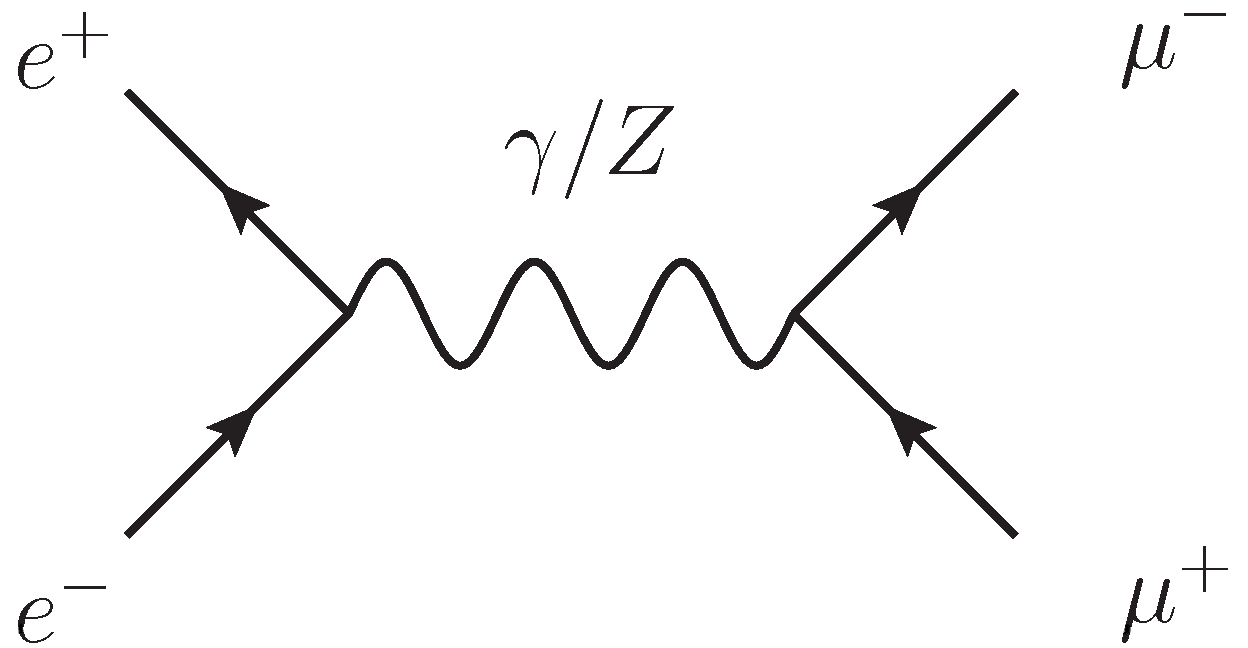
\includegraphics[width=0.7\textwidth]{Feynman_diagrams/Jaxo_annihilation.png}
     \caption{Direct annihilation}
     \end{subfigure}
    \caption[Muon production processes]{
    Feynman diagrams of the muon pair production via the Bethe-Heitler process and the direct annihilation with atomic electrons.}
    \label{fig:BDS_Muons:Muon_production}
\end{wrapfigure}
To prevent the muons from reaching the detectors, two different shielding systems are studied with respect to their effectiveness and feasibility to be integrated in the BDS.
Both systems are based on two ideas: to deflect the muons such that they do not reach the interaction region, and also to stop the muons in the shielding material.
The shielding scenarios that are under discussion foresee a combination of the two systems:
\begin{itemize}
 \item ``5 spoilers'':\\
 In the first scenario, five cylindrical spoilers out of magnetized iron are installed at different locations along the BDS: \SI{1358.5}{\metre}, \SI{1234.5}{\metre}, \SI{1145.5}{\metre}, \SI{975.5}{\metre}, and \SI{802.5}{\metre} from the interaction point (IP), where these locations indicate the midpoint of the spoiler.
 \\The spoilers have a radius of \SI{70}{\centi\meter}, and a length of about \SI{5}{\meter}.
 Their magnetic field ranges from about \SI{19}{\kilo\gauss} in the center of the spoiler to about \SI{10}{\kilo\gauss} at the outer edge~\cite{MuonShielding,Lewis}.
 An illustration of one of these spoilers is given in Figure~\ref{fig:BDS_Muons:shielding_options} (a).
 As indicated by the muon tracks through the spoiler, the magnetic field of the cylindrical spoilers is such that either positively or negatively charged muons are deflected away from the beam path into the tunnel walls.
 \item ``5 spoiler + wall'':\\
 In the second scenario, the same five spoilers are located at the same positions as before.
 But an additional magnetized shielding wall is placed about \SI{400}{\meter} from the interaction point.
 \\The wall is about \SI{5}{\meter} wide and long, and fills out the complete tunnel height.
 Its magnetic field strength is about \SI{16}{\kilo\gauss}~\cite{MuonShielding,Lewis}.
 Figure~\ref{fig:BDS_Muons:shielding_options} (b) shows an illustration of the wall inside the BDS tunnel.
\end{itemize}
The motivation for the study presented in this section is to investigate the effect of the muons on the SiD detector.
The overall goal is to give a recommendation, based on the study of the detector performance, on the necessity of the magnetized in order to keep the detector occupancy below the critical limit of \num{e-4} (as discussed in previous chapters).
Arguments against the wall were brought forward regarding costs and safety issues due to its size in the BDS tunnel.
 \begin{figure}
 \centering
  \begin{subfigure}[b]{0.49\textwidth}
   \centering
    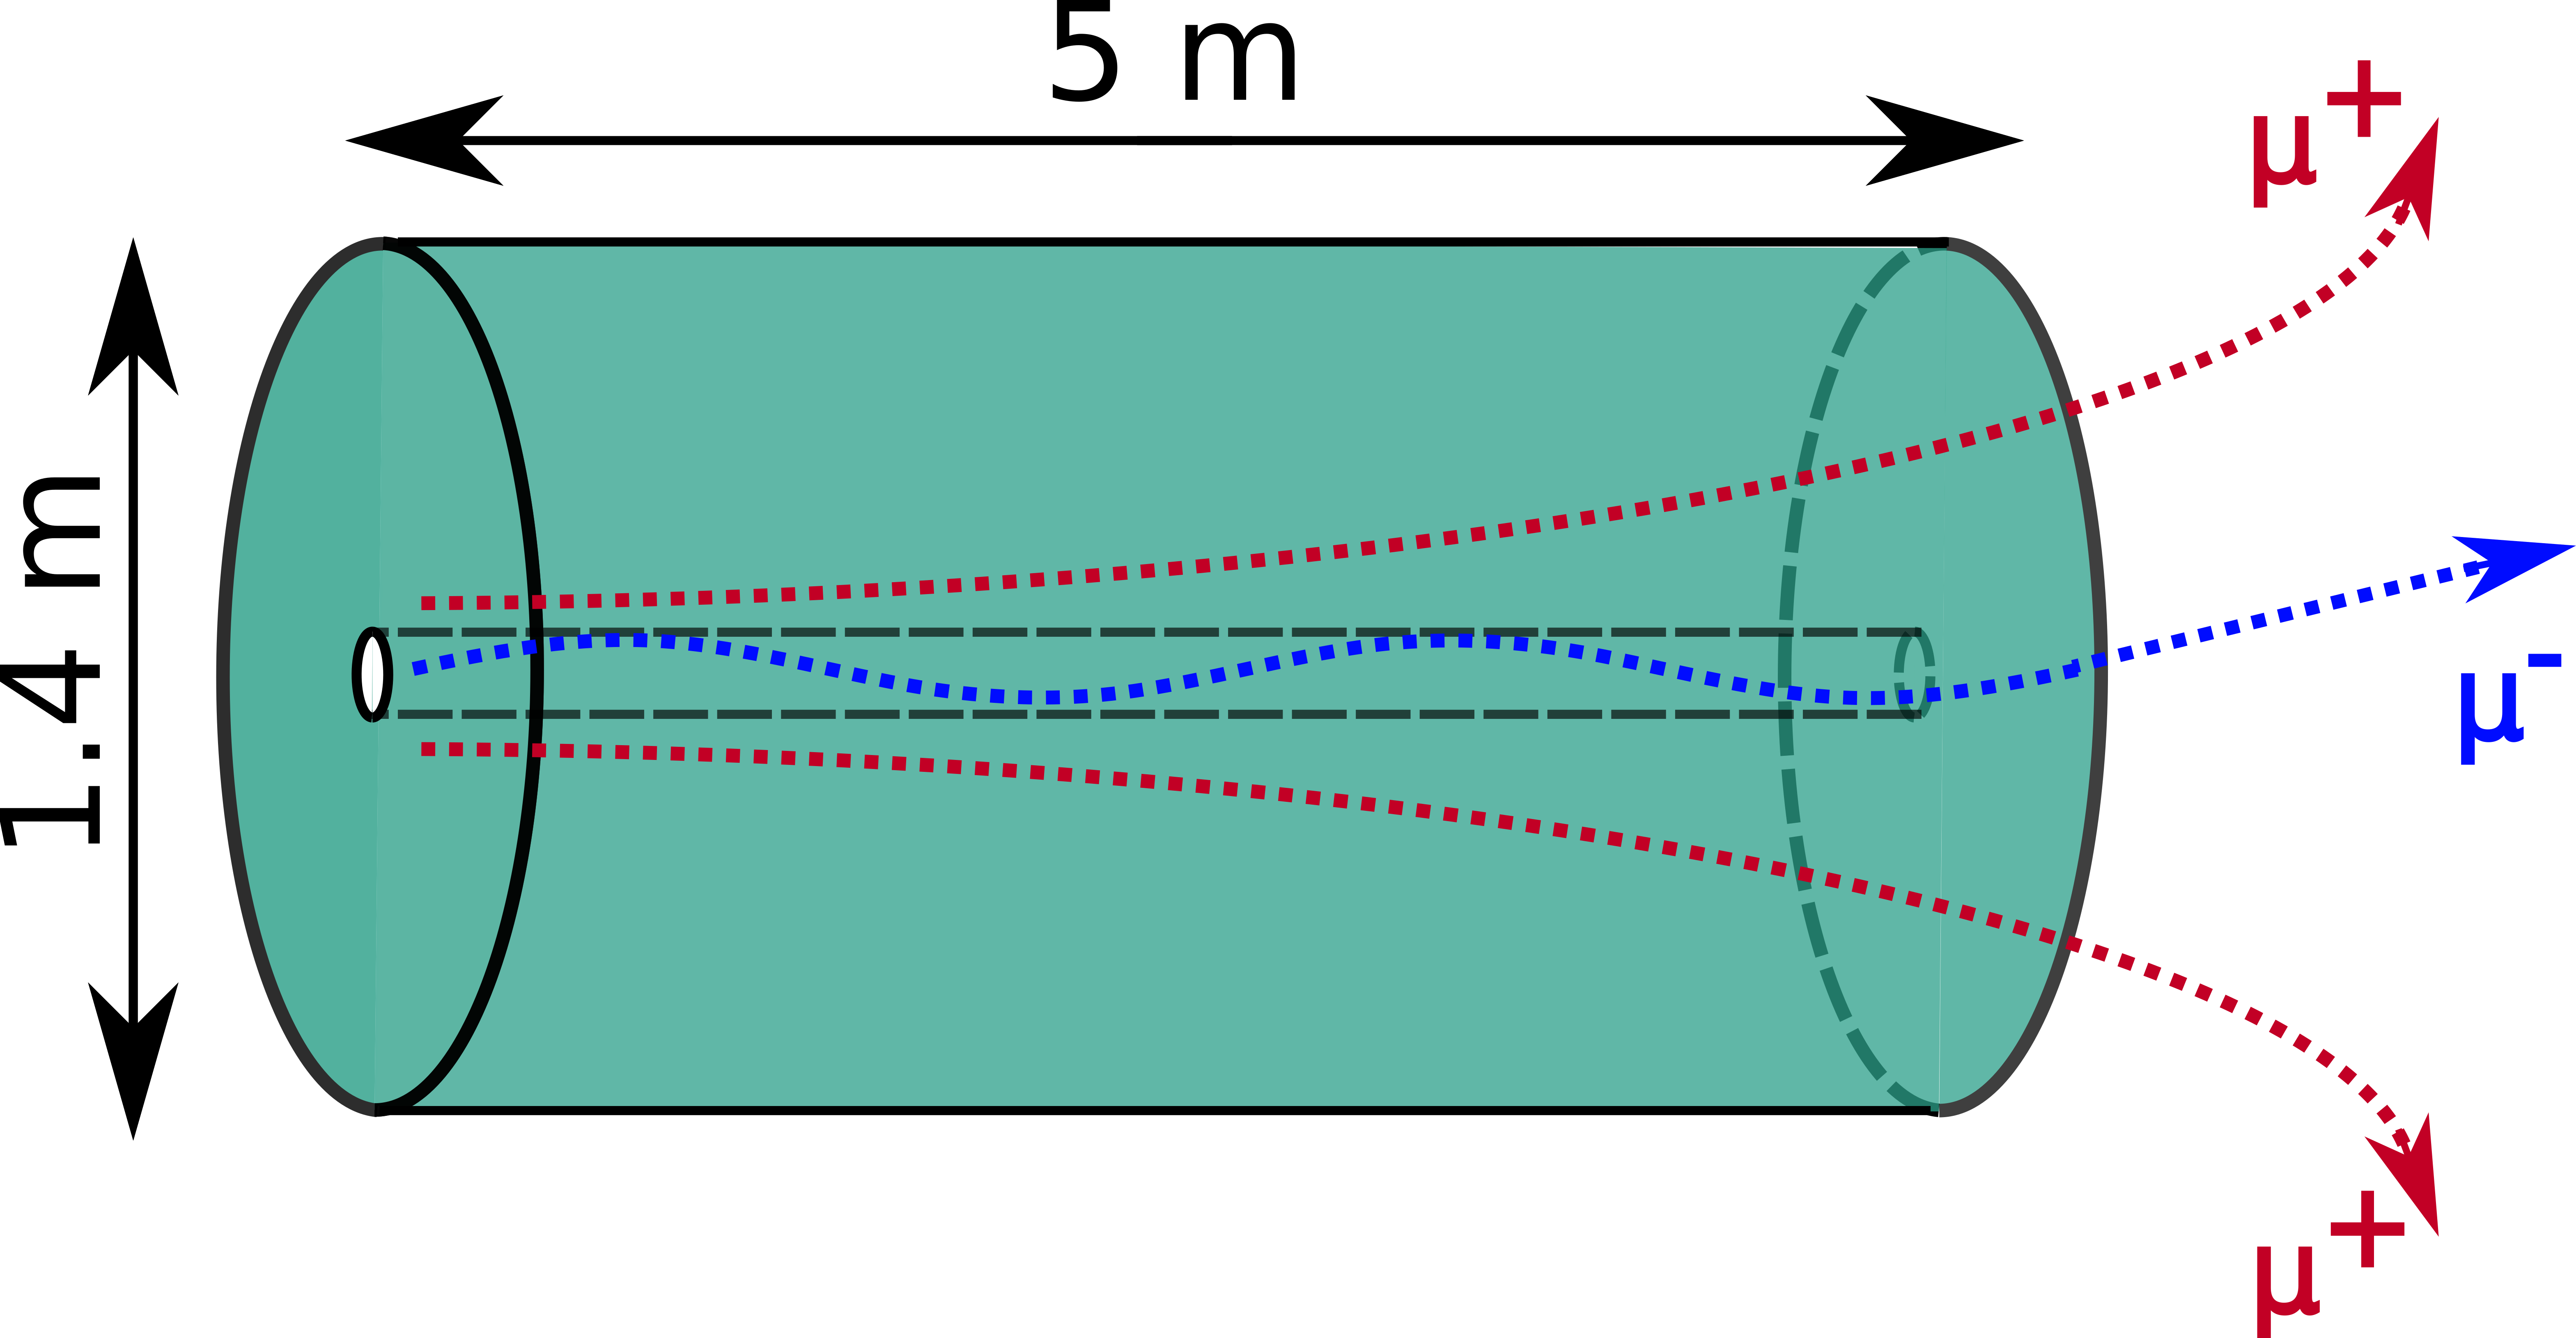
\includegraphics[width=0.7\textwidth]{Figures/BDS_muons/spoilers.png}
   \caption{Cylindrical spoiler}
   \label{fig:spoilers}
   \end{subfigure}
   \hfill
    \begin{subfigure}[b]{0.49\textwidth}
   \centering
    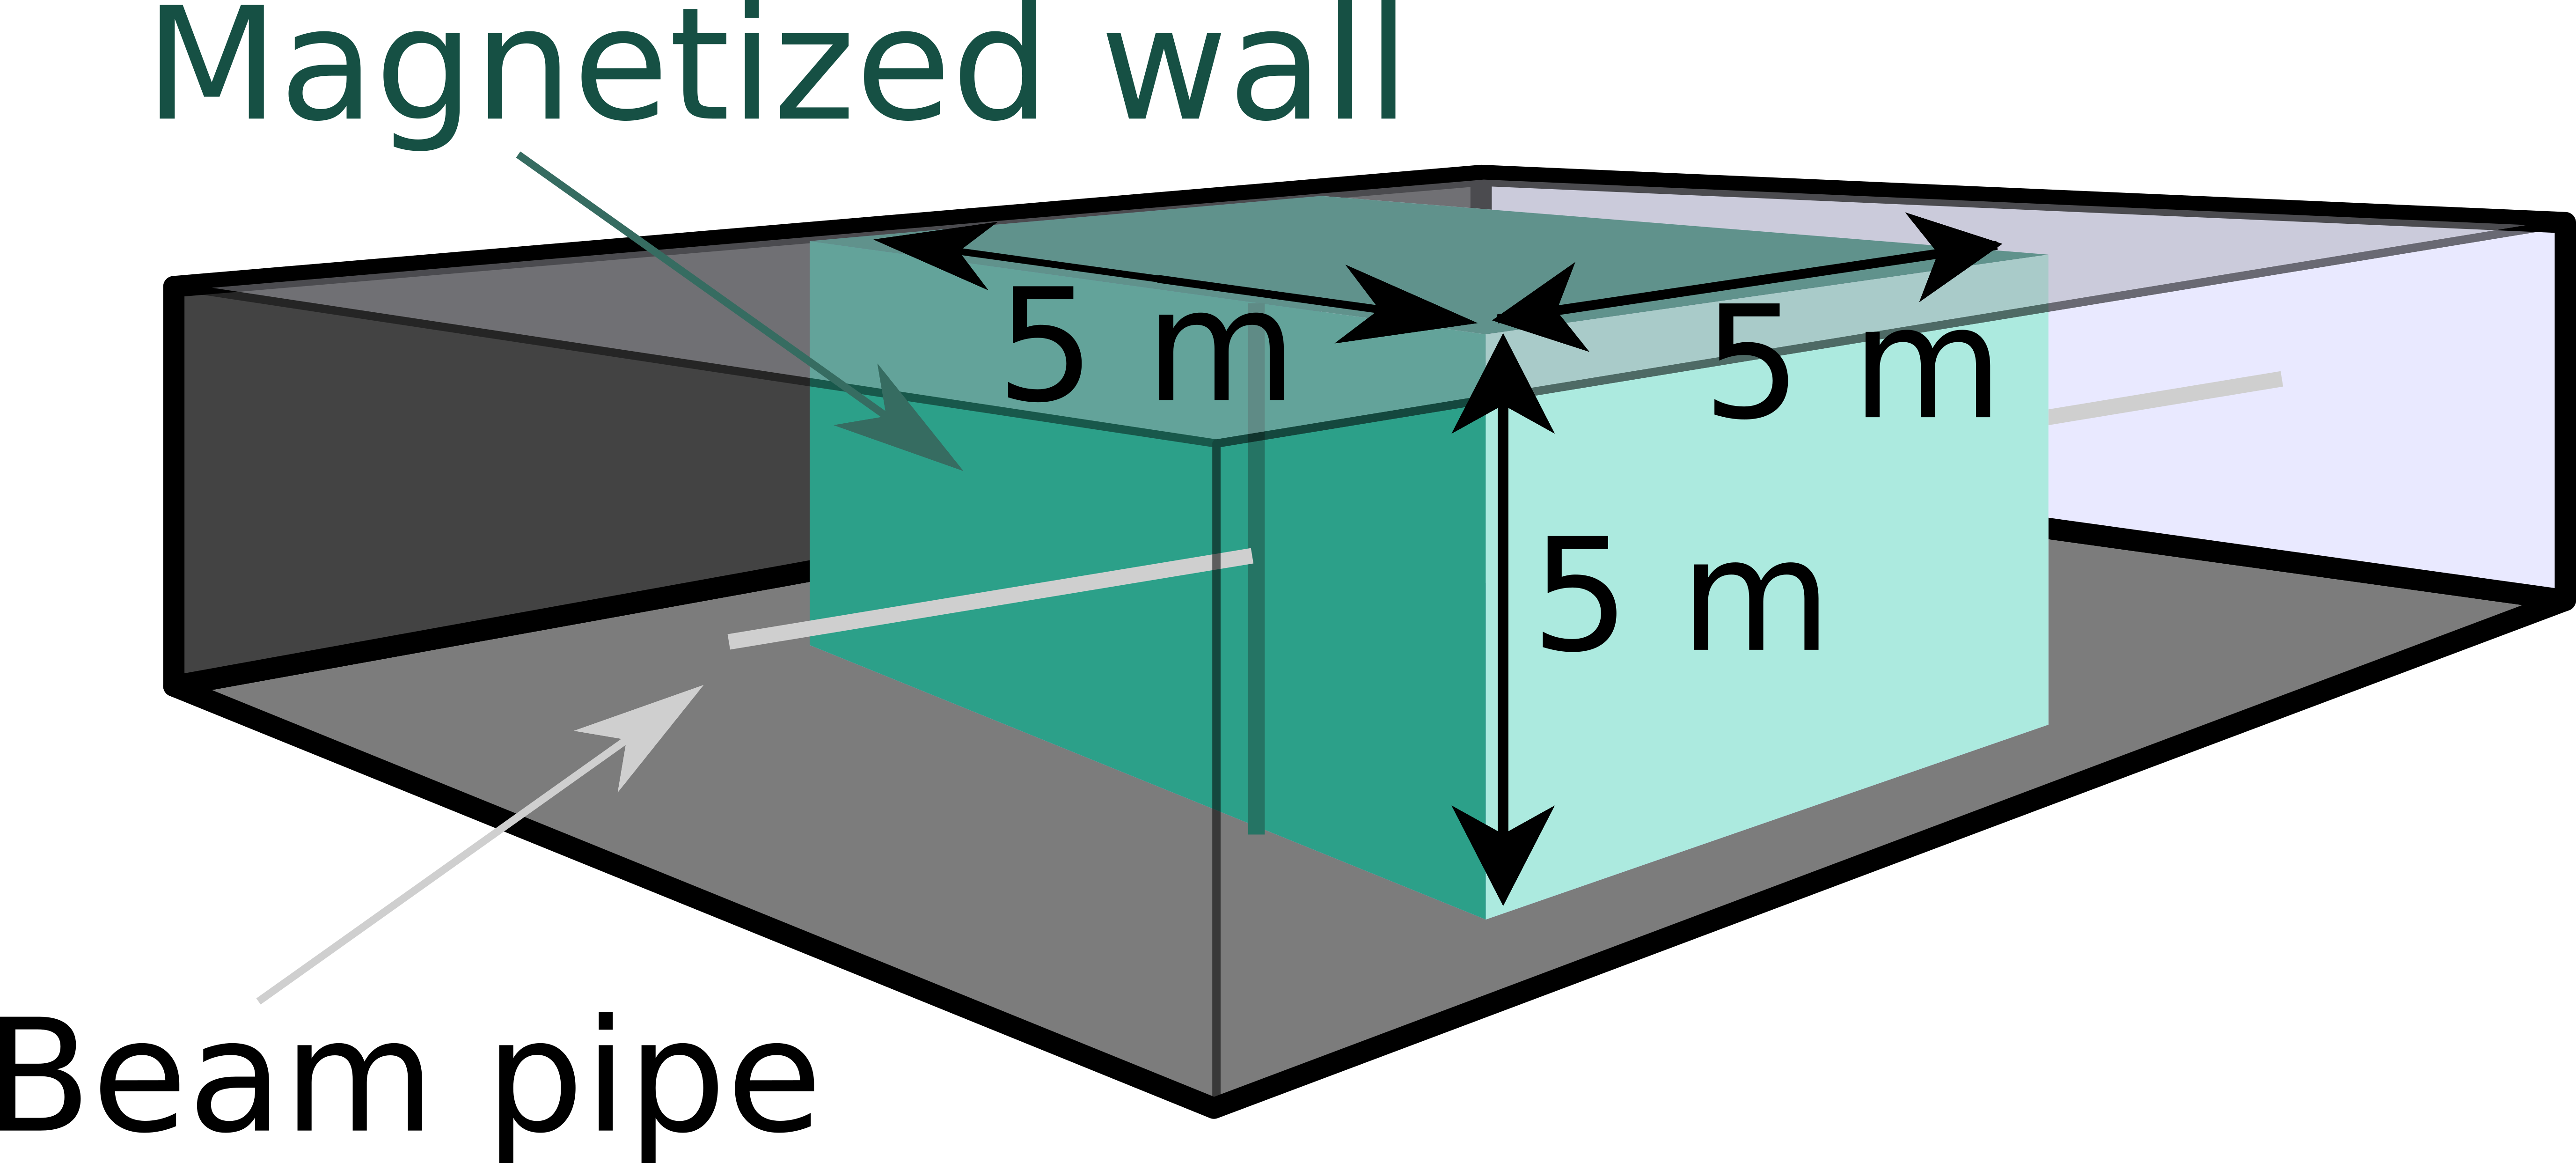
\includegraphics[width=\textwidth]{Figures/BDS_muons/muon_wall.png}
   \caption{Magnetized wall}
   \label{fig:muon_wall}
   \end{subfigure}
   \caption[BDS muon shielding options]{Schematic drawings of the magnetized spoiler (a) and the magnetized shielding wall (b)~\cite[cf. p. 2]{MuonShielding}.
   The magnetized wall is illustrated inside the accelerator tunnel.}
   \label{fig:BDS_Muons:shielding_options}
 \end{figure}

\subsection{\mucarlo}
\label{BDS_Muons:MUCARLO}
The interactions between the ILC beam and the machine components in the BDS were simulated with a Monte Carlo tool called \mucarlo~\cite{Mucarlo,MuonBkg_05TeV,MuonBkg_1TeV}.
Since the presented study is done for two different ILC stages, at \SI{250}{\GeV} and at \SI{500}{\GeV}, the beam parameters of the respective stage were used accordingly.
The geometry lattice of the ILC Beam Delivery System serves as the input geometry to the \mucarlo code, through which the muons are tracked.
Figure~\ref{fig:BDS_Muons:tracks} shows the muon tracks in the electron-line of the BDS.
The muons are created at certain locations along the beam line, are deflected by the magnetic field of beam line components, and lose kinetic energy through scattering in the material of the components the muons hit.
In the end, only those muons that reach the IP (at z = \SI{0}{\meter}) are stored.
Accordingly, Figure~\ref{fig:BDS_Muons:tracks} only shows those muons.
In this plot, there is only one red muon track line, which belongs to a negatively charged muon.
The spoiler polarities are set to defocus muons with the same charge as the beam charge.
Therefore, mainly positively charged muons from the electron beam line will reach the IP.
For the positron beam line, the muons reaching the IP are mainly negatively charged.
\\The main sources of muons were identified in the BDS to be 11 distinct collimators.
The following list names these collimators and their position from the IP~\cite{Lewis}:
\begin{itemize}
 \item Primary collimator spoilers (radiation length: 0.6 X\textsubscript{0}, half-gap\footnote{The term ``half-gap'' is commonly used for collimator systems.
 It describes the gap between one of the collimator jaws and an arbitrarily chosen plane (usually the beam center plane).
 Both of the jaws have the same distance from this plane.}: \SI{930}{\micro\meter} in x, \SI{400}{\micro\meter} in y):\\
  SP2 (\SI{1508}{\meter}), SP4 (\SI{1332}{\meter})
 \item Protection collimators (radiation length: 30 X\textsubscript{0}, inner radius: \SI{0.7}{\centi\meter}):\\
  PC1 (\SI{1452}{\meter}), PC2 (\SI{1387}{\meter}), PC5 (\SI{1276}{\meter}), PC5A (\SI{1242}{\meter}), PC6 (\SI{1208}{\meter}), PC7 (\SI{1047}{\meter})
 \item Absorbers (radiation length: 30 X\textsubscript{0}, half-gap: \SI{0.7}{\centi\meter}):\\
  AB3 (\SI{1420}{\meter}), AB5 (\SI{1237}{\meter}), ABE (\SI{852}{\meter})
\end{itemize}
The protection collimators and absorbers serve the purpose of protecting the magnets of the BDS from particle showers (arising from the beam halo collimation) and from mis-steered primary beams.
The number of muons created is proportional to the fraction of the collimator surface that is hit with respect to the beam size, which was determined with the help of the Monte Carlo ray-tracing computer program \turtle~\cite{Turtle}.
The general design of these collimators can be found in \cite{BDS_coll_design}.
\begin{figure}
\centering
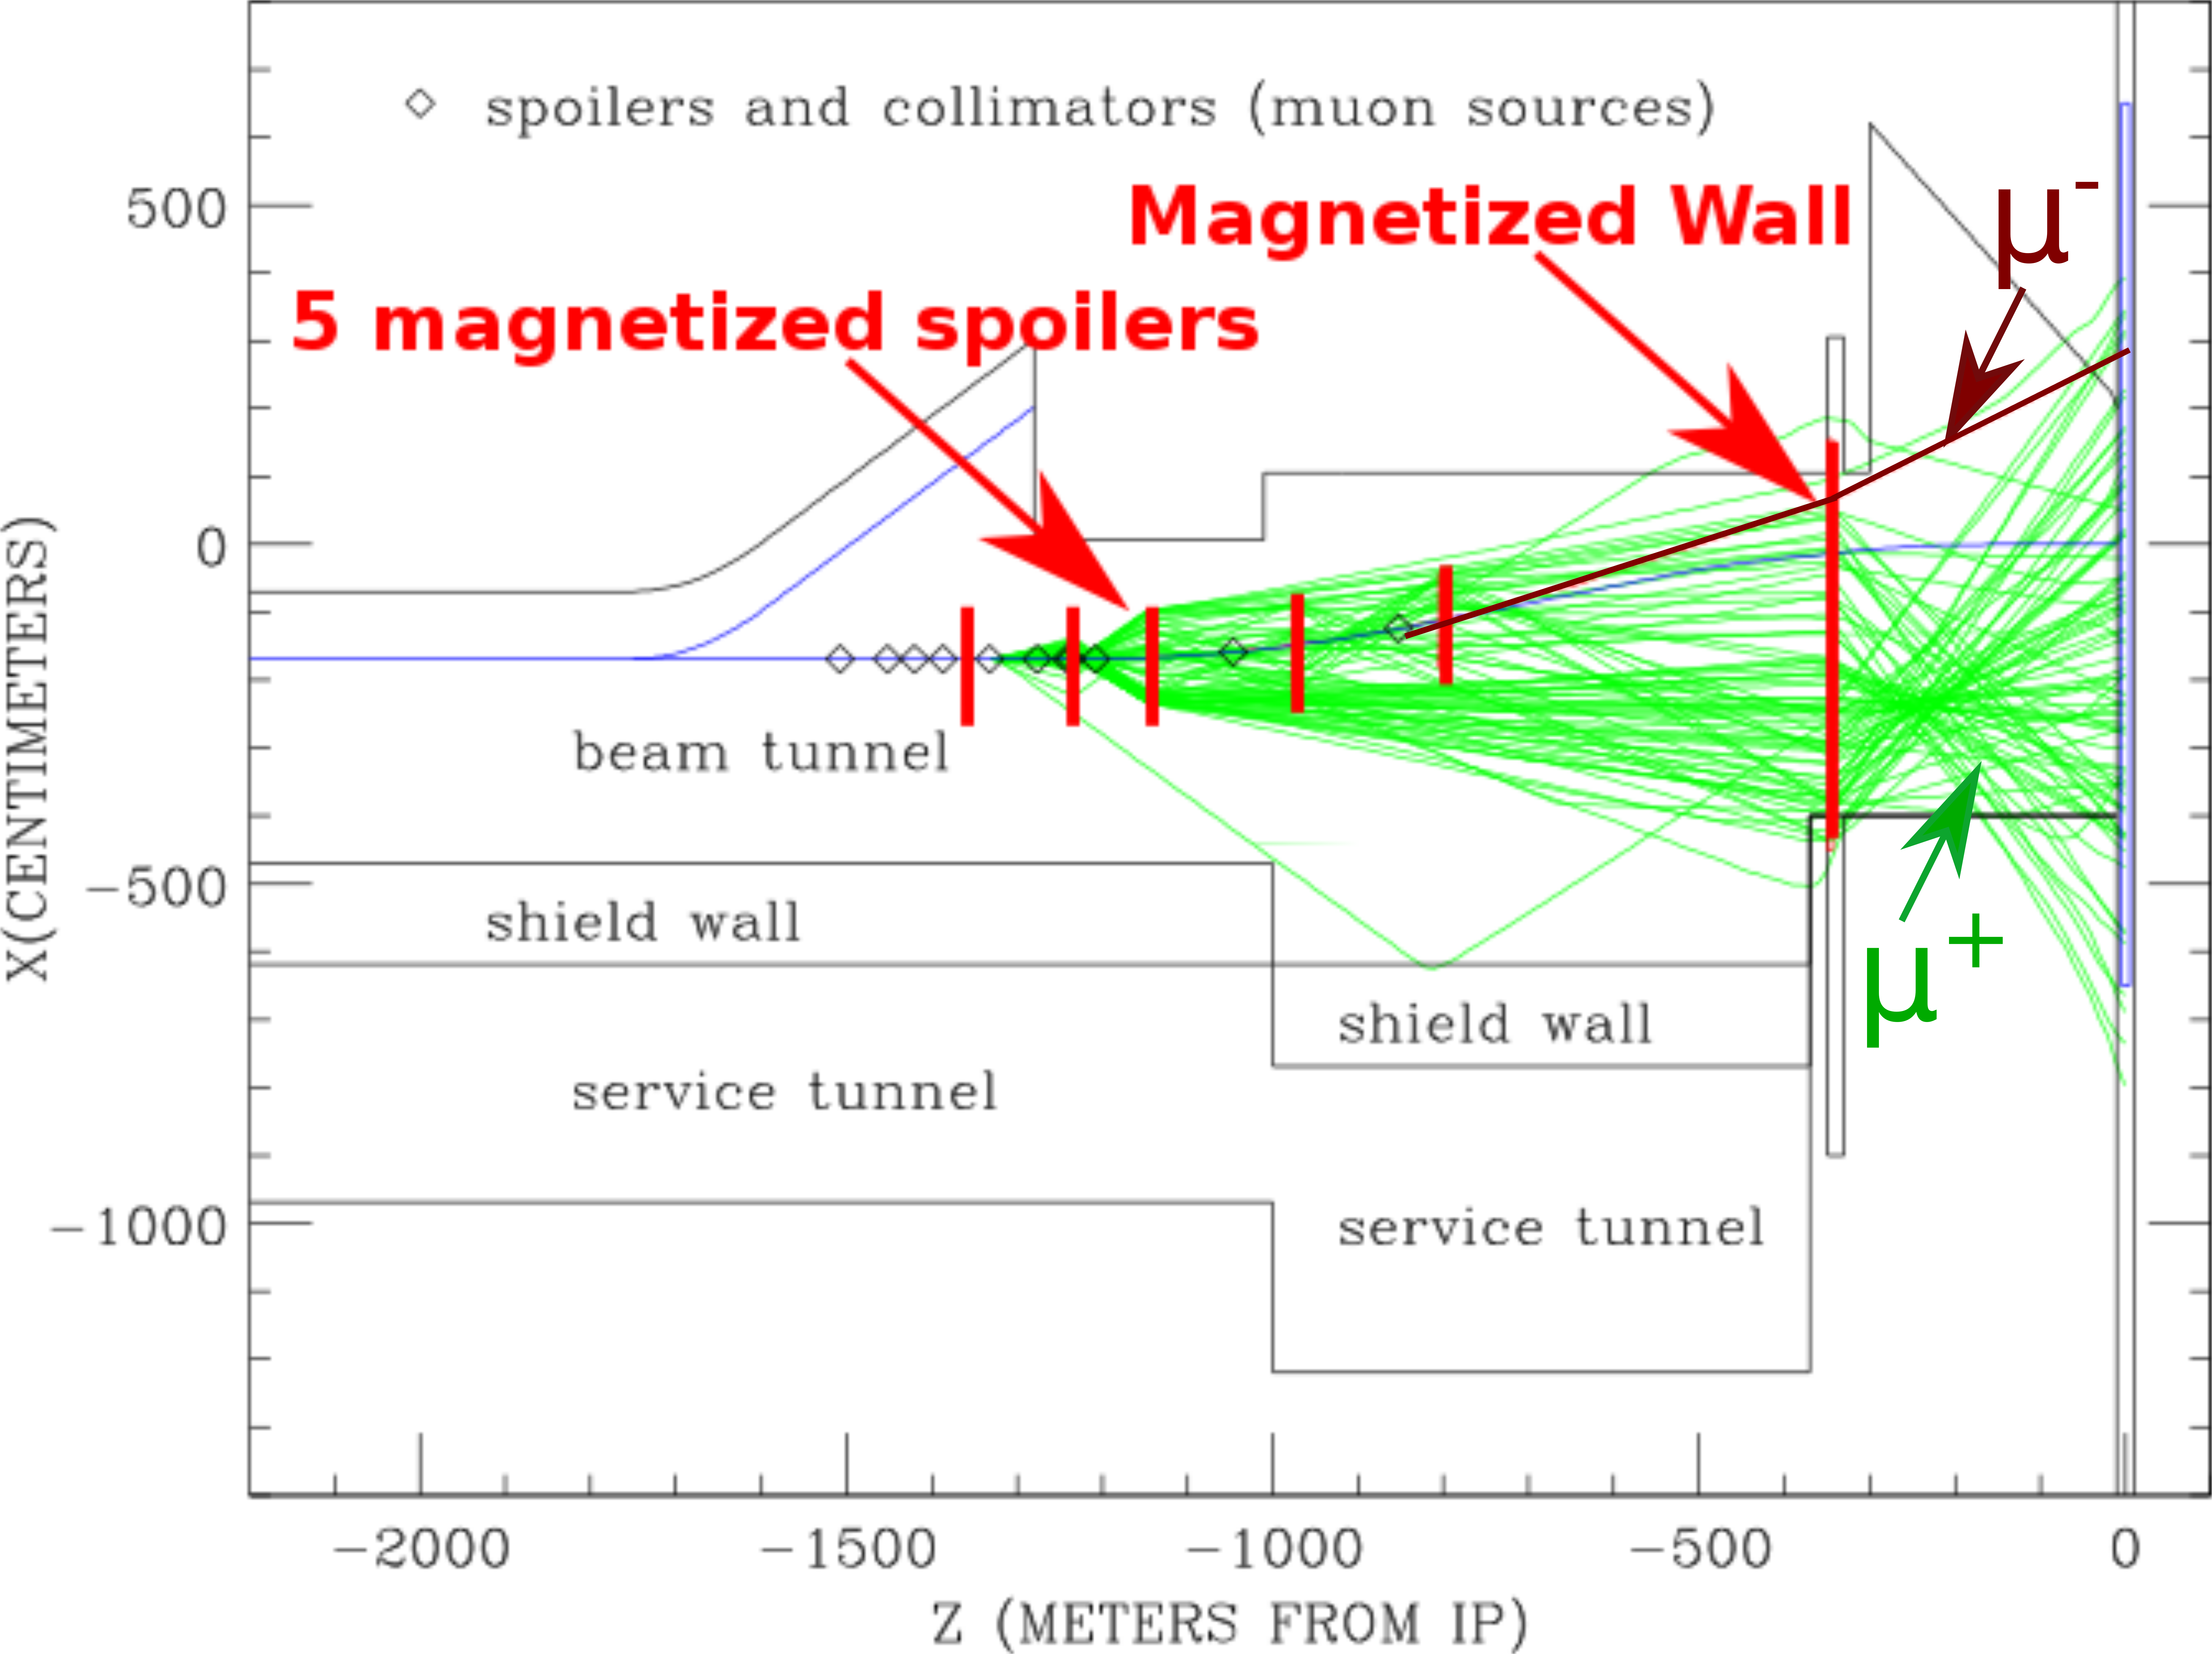
\includegraphics[width=0.6\textwidth]{Figures/BDS_muons/BDS_Tunnel_Spoilers+Wall_edited.png}
\caption[Muon tracks in the Beam Delivery Systems]{Visualization of the muon tracks in the ILC Beam Delivery System (BDS)~\cite{Lewis}.
The picture shows the xz-plane of the BDS tunnel with the beam line components (spoilers and collimators), which serve as muon sources.
In this particular example, the muons origin from the primary collimator spoiler SP4.
The locations of the muon shielding components (the magnetized spoilers and wall) are also indicated.
The green/red thin lines represent the tracks of the muons.}
\label{fig:BDS_Muons:tracks}
\end{figure}
Adding up all muons from the different sources on the electron and the positron beam line side, the total number of muons can be calculated that would reach a detector with a radius of \SI{6.5}{\meter} at the interaction region.
Table~\ref{tab:BDS_Muons_muon_numbers} lists the muon rates per bunch crossing for a center-of-mass energy of 250 and \SI{500}{\GeV}, and for the two different shielding scenarios.
At \SI{500}{\GeV}, about 130 muons per bunch crossing would reach the detector in the case that no shielding was installed.
This number is reduced to about 4 muons with the five cylindrical spoilers, and to below 1 muon per bunch crossing with an additional magnetized wall.
For a lower beam energy of \SI{125}{\GeV} (\SI{250}{\GeV} center-of-mass energy), the number of muons that are produced is lower, because of which only around 38 muons reach the detector without shielding.
With the two different shielding scenarios, the muon rate is again reduced significantly to a minimum of about 0.03 per bunch crossing.
%------------------
%\newcolumntype{L}[1]{>{\raggedright\let\newline\\\arraybackslash\hspace{0pt}}m{#1}}
%\newcolumntype{C}[1]{>{\centering\let\newline\\\arraybackslash\hspace{0pt}}m{#1}}
%\newcolumntype{R}[1]{>{\raggedleft\let\newline\\\arraybackslash\hspace{0pt}}m{#1}}
%-----------------
\begin{table}[htbp]
\caption[\mucarlo muon rates]{Muon rates per bunch crossing for the two shielding scenarios, gained from \mucarlo simulations~\cite{Lewis}.}
\label{tab:BDS_Muons_muon_numbers}
\centering
\begin{tabularx}{0.56\textwidth}{l|C{3cm}|C{3cm}}
\hline\hline
\textbf{Scenario} & \multicolumn{2}{>{\centering}p{6cm}}{\textbf{Muons per bunch crossing in a detector with 6.5\,m radius}}\\
& ILC500 & ILC250\\
\hline
 No Spoilers & 130 & 38\\
 5 spoilers& 4.3 & 1.3\\
 5 spoilers + wall & 0.6 &  0.03\\
\hline\hline
\end{tabularx}
\end{table}
\\The output of \mucarlo is a text file containing the four-vectors of the muons \SI{10}{\meter} from the IP.
These four-vectors can therefore be used as input to a full detector simulation. 
\\An additional study was done using a \geant simulation of the BDS tunnel in order to cross check the \mucarlo results and to thereby verify the \mucarlo simulation.
The outcome of that study was that both simulations are in good agreement~\cite{Glens_muon_talk}.

\subsection{Effect of muons on the SiD performance}
\label{BDS_Muons:SiD}
Since the SiD detector only reads out the hits after every bunch train (1312 bunch crossings), the detector occupancy for the muons has to be studied for a muon rate per train.
As in the previous chapter, the full detector simulation was done using \slic.
The geometry input file that was used contained the most recent sidloi3 geometry of the SiD detector, including the new L* position, the anti-DiD field, as well as the Pacman geometry.
For details on these detector characteristics, please refer to Section~\ref{ILC:SiD}.
After a file-format conversion, the \mucarlo output files containing the four-vectors of the muons for the different shielding scenarios and center-of-mass energies served as the particle source input to \slic.

\subsubsection{Muon hit distribution}
For visualizing the hit distribution in the SiD detector, event displays (see Figure~\ref{fig:BDS_Muons:wired4}) were made using WIRED4~\cite{Wired4}.
 \begin{figure}[htbp]
 \centering
  \begin{subfigure}[b]{0.31\textwidth}
   \centering
   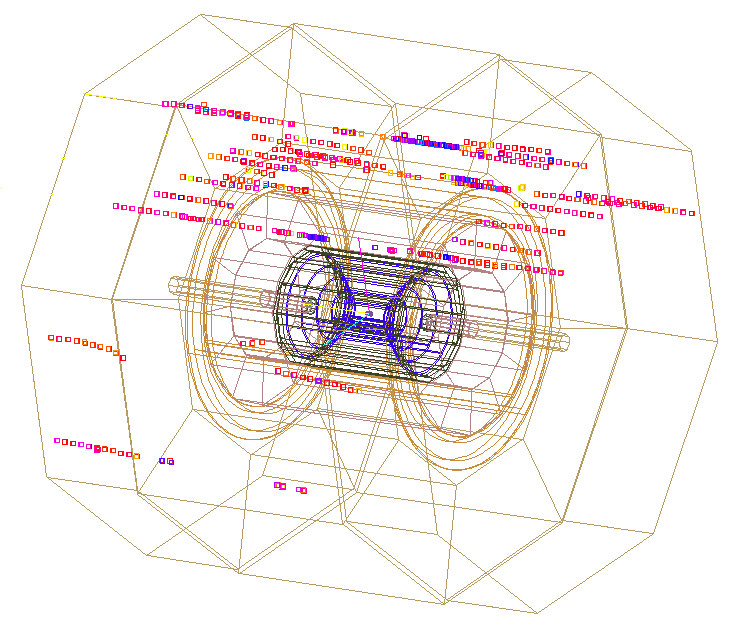
\includegraphics[width=\textwidth]{Figures/BDS_muons/Event_display_ILC250_p_spoilers_wall_inverted.png}
   \caption{3D view, 5 spoilers + wall,\\ILC250}
   \end{subfigure}
   \hfill
   \begin{subfigure}[b]{0.31\textwidth}
   \centering
    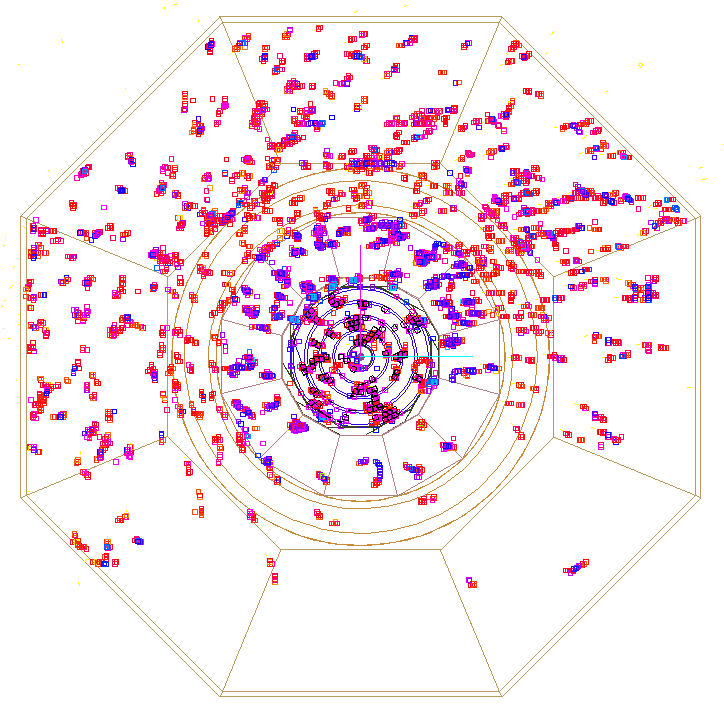
\includegraphics[width=0.9\textwidth]{Figures/BDS_muons/muons_positron_5spoilers_wall_515_xyview_croped_inverted.png}
   \caption{xy-view, 5 spoilers + wall,\\ILC500}
   \end{subfigure}
   \hfill
    \begin{subfigure}[b]{0.31\textwidth}
   \centering
    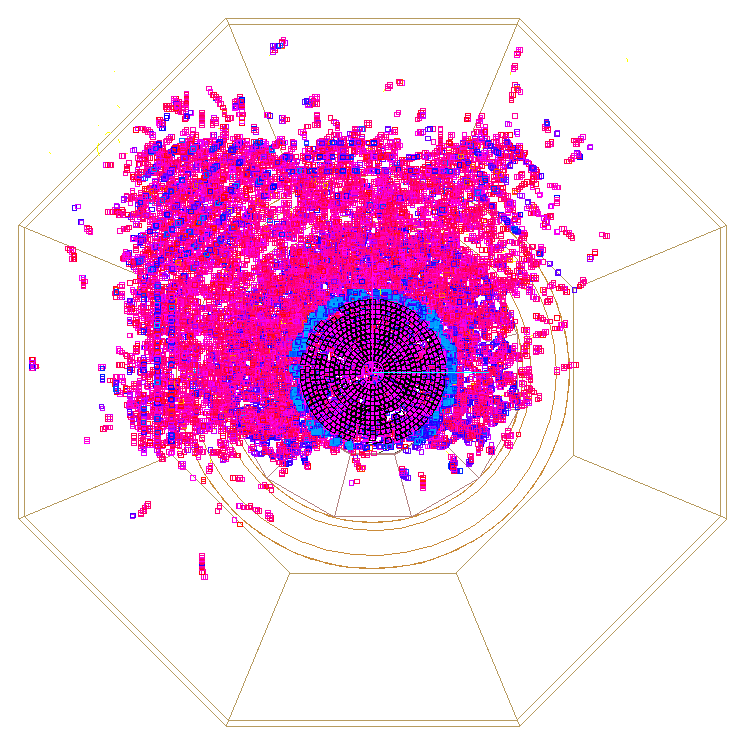
\includegraphics[width=0.9\textwidth]{Figures/BDS_muons/muons_positron_5spoilers_2961_xyview_croped_inverted.png}
   \caption{xy-view, 5 spoilers,\\ILC500}
   \end{subfigure}
   \caption[Event displays of BDS muons in SiD]{Event displays of the muon hits in SiD for different center-of-mass energies and different shielding scenarios.}
   \label{fig:BDS_Muons:wired4}
 \end{figure}
\\Apart from the overall number of hits in the different event displays, the spatial distribution of the hits is striking.
Concentrating on Figure~\ref{fig:BDS_Muons:wired4} (a) first, the muons leave clear horizontal tracks throughout the whole detector.
After leaving the BDS tunnel, the muons (which are boosted in forward direction) enter SiD through the outermost subdetector, and penetrate the full detector.
Since the muons are coming from both the electron and the positron beam line, this happens simultaneously from both sides.
\\The difference in the spatial distribution in the xy-plane between Figure~\ref{fig:BDS_Muons:wired4} (b) and (c) is explained by the geometry of the tunnel, and position of the detector with respect to the tunnel exit.
In subfigure (a), the rectangular shape in the hit distribution is the imprint of the tunnel.
The boosted muons exit the tunnel and directly hit the detector.
The asymmetry of the imprint results from the position of the detector.
The beam pipe and therefore the central axis through the detectors are not in the center of the BDS tunnel.
As can be seen in Figure~\ref{fig:BDS_Muons:tracks}, the beam line curves such that it is closer to one of the tunnel side walls than to the other.
The top-bottom asymmetry is due to the fact that the detector cavern is below ground level of the tunnel.
\\Adding the magnetized wall as an additional muon shielding causes the muons to scatter.
The clear tunnel imprint is no longer visible in Figure~\ref{fig:BDS_Muons:wired4} (b).
Scattering the muons is not the only effect of the magnetized wall.
As can be seen in Figure~\ref{fig:BDS_Muons:energy}, the wall shifts the muon energy to lower values for a respective center-of-mass energy.
The muons are deflected away from the forward directions due to the magnetization of the wall, but also lose their energy in the material of the wall.
Low energy muons are either stopped completely, or deflected such that they cannot reach the detector. %\todo{Check out Bethe-Bloch here}
The peak in the energy distributions at lower energies is therefore reduced for the ``5 spoilers + wall'' scenarios.
Additionally, the number of muons per bunch train can directly be compared for the two ILC stages and the different shielding options.
\begin{figure}[htbp]
\centering
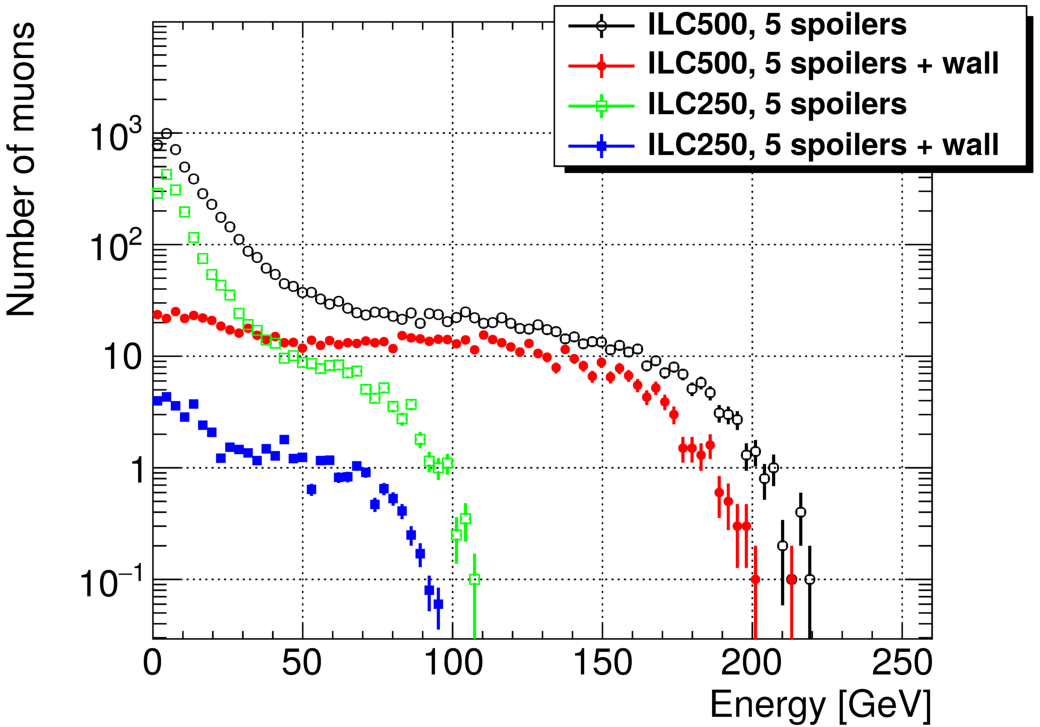
\includegraphics[width=0.6\textwidth]{Figures/BDS_muons/Energy_Comparison_ILC500vsILC250.pdf}
\caption[Muon energy]{Energy distribution of the muons for the different shielding scenarios, and for a center-of-mass energy of 250 and \SI{500}{\GeV}.
The number of muons are normalized to a full bunch train for all cases.}
\label{fig:BDS_Muons:energy}
\end{figure}
\\These muons then leave a particular number of hits in the SiD subdetectors by penetrating the full detector.
For the comparison between the total number of hits in the four different cases, Figure~\ref{fig:BDS_Muons:hits} shows a bar chart of the hits collected in each subdetector.
The largest number of hits is counted for the endcaps of the muon detector system, which is the subdetector with the largest effective detector area under normal incident of the muons.
Also, it is the outermost subdetector, likely to be hit by all of the primary muons.
Accordingly, the vertex detector (as the smallest and innermost detector) is hit the least number of times, and in the same manner also the other subdetectors gain representative number of hits.
Deducing from the hit distributions, the SiD detector will overall suffer from less hits in the ILC250 stage with respect to the ILC500, but adding the magnetized wall to the shielding will yield even smaller hit counts for both center-of-mass energies.
\begin{figure}[h]
\centering
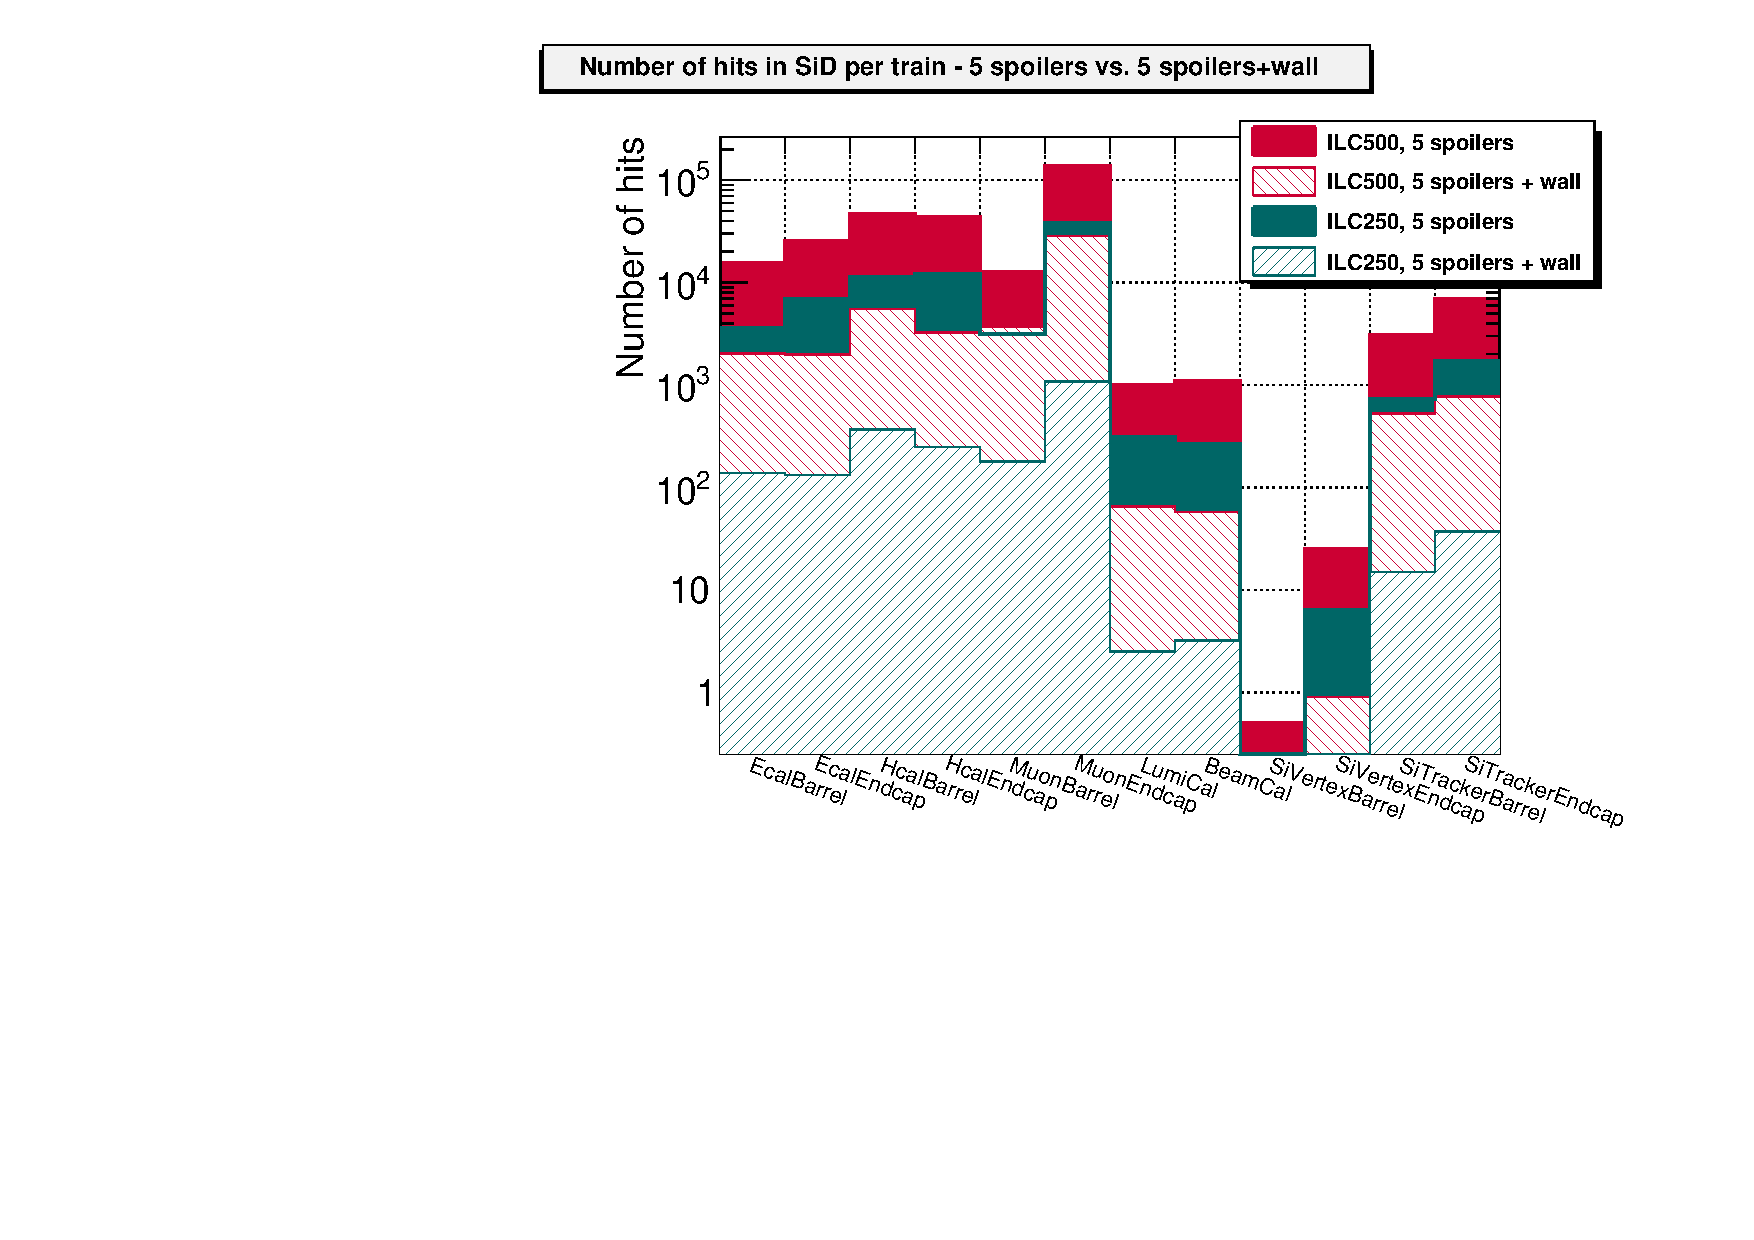
\includegraphics[width=0.7\textwidth]{Figures/BDS_muons/Hits_in_SiD_subdetectors_MuonSpoilerStudy.pdf}
\caption[Number of muon hits in the SiD subdetectors]{Total number of hits in the various SiD subdetectors for both shielding scenarios and both ILC stages.
The number of hits come from muons from a full bunch train.}
\label{fig:BDS_Muons:hits}
\end{figure}
\\After looking at the total number of hits, which reflects the size and position of the subdetectors in SiD, this fact can be even better derived from the hit time distributions shown in Figure~\ref{fig:BDS_Muons:hittime}.
The muons emitted from the BDS tunnel arrive first at the endcaps of the muon system, as mentioned above.
After penetrating all muon endcap layers, the next outermost subdetector is hit and so on, until the muons make their way to the opposite muon endcap.
The time needed for the muons to penetrate the full detector is hence about \SI{40}{\nano\second}, independent of the muon shielding and the center-of-mass energy.
\begin{figure}[htbp!]
\centering
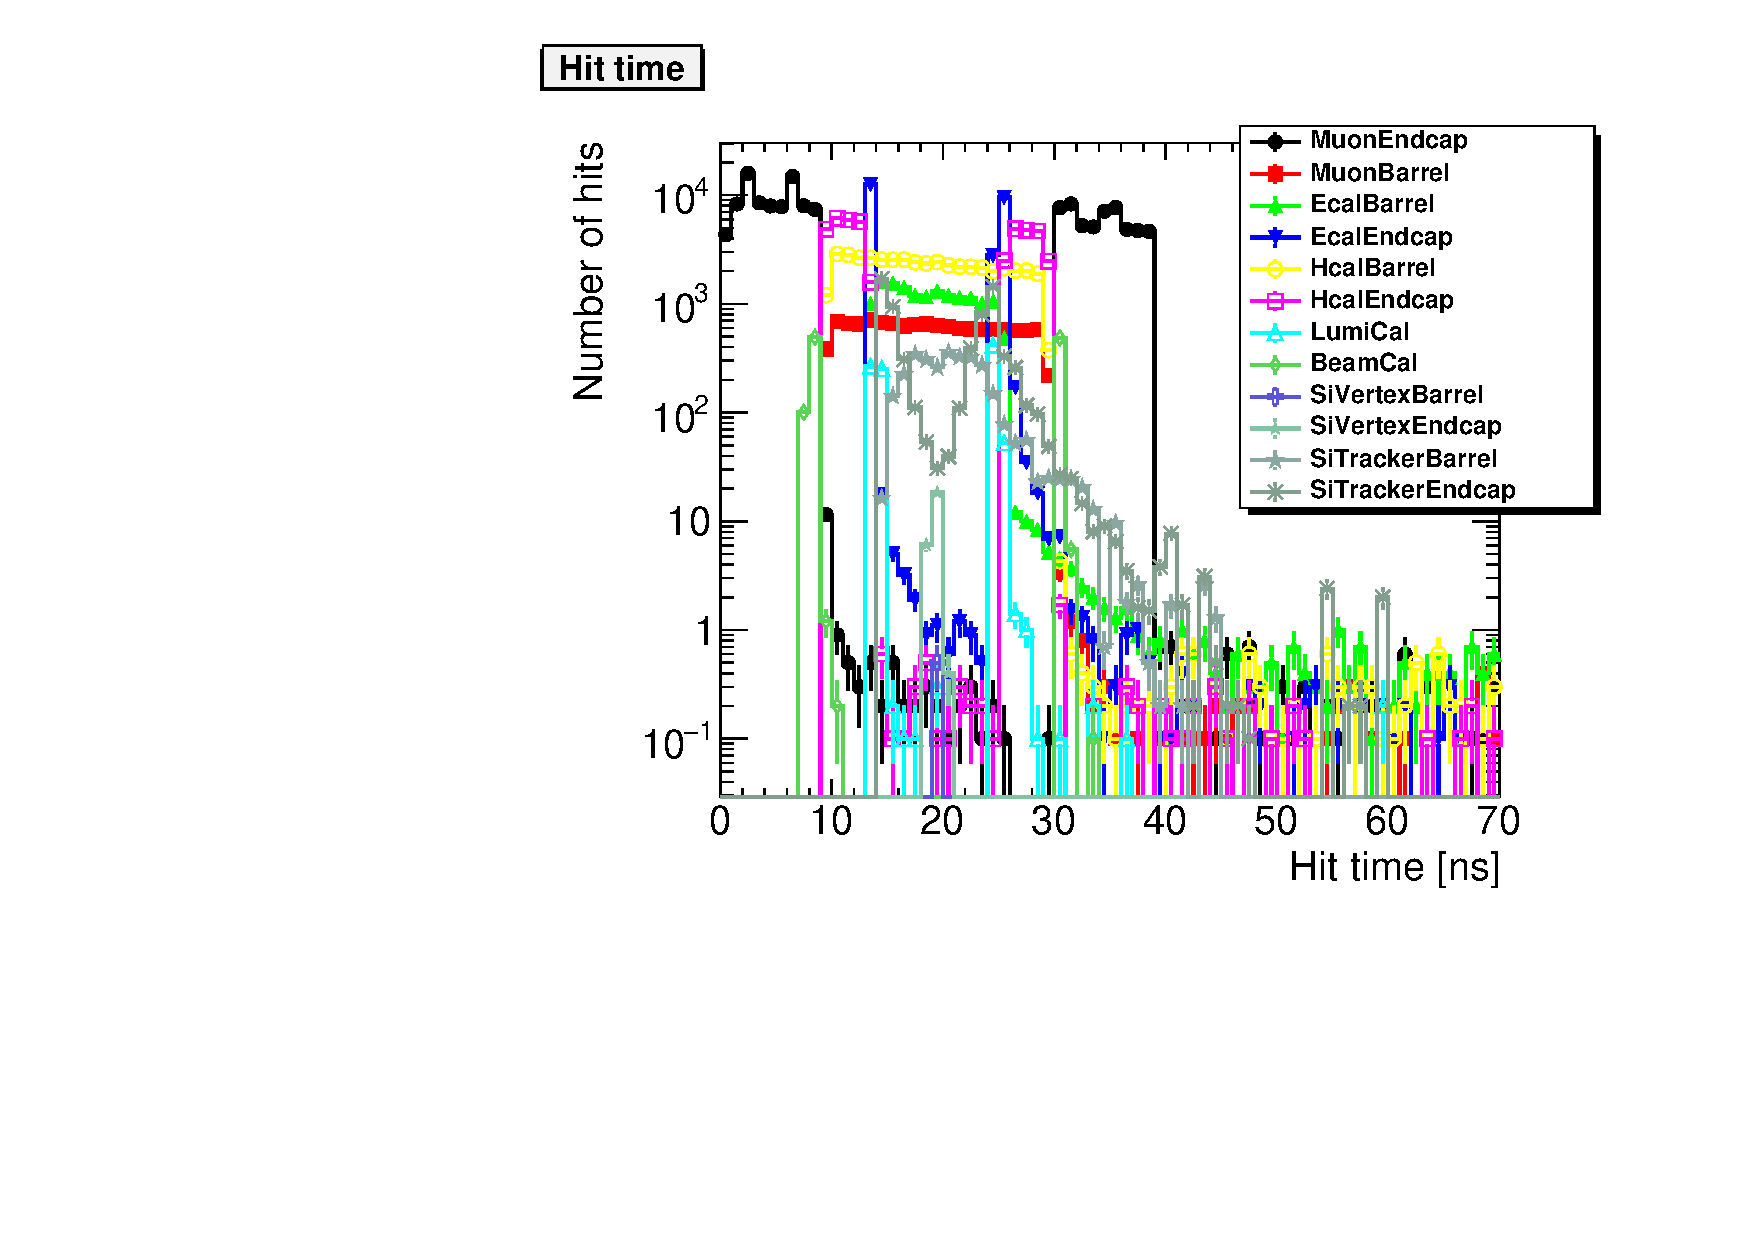
\includegraphics[width=0.7\textwidth]{Figures/BDS_muons/hittime_ILC500_spoilers_superimposed.pdf}
\caption[Muon hit time in the SiD subdetectors]{Hit time distribution of the BDS muons in the various SiD subdetectors for ILC500 stage and for the ``5 spoilers'' scenario only.
The number of hits are normalized to hits from a full bunch train for all cases.}
\label{fig:BDS_Muons:hittime}
\end{figure}

\subsubsection{SiD occupancy}
The next step is to look at the occupancy of the detector arising from these muon hits.
As in Chapter~\ref{PairBkg:occupancy}, the number of hits are counted for every cell in the subdetectors, which can be directly translated into a detector occupancy.
In the following, the muon occupancy in the SiD HCAL barrel and the tracker endcaps is discussed.
As explained in the previous chapter, occupancy plots show how many detector cells are hit a certain number of times. 
By respecting the rule that the sum of all cells with a number of hits greater than or equal to the buffer depth should not exceed \SI{0.01}{\percent} (\num{e-4} of all cells), a statement can be made whether given occupancy levels are acceptable.
By optimizing the design of the detectors and the accelerator, a balance can be found between a sufficient buffer depth of the detector sensors and low background levels arising from the accelerator.
\\Figure~\ref{fig:BDS_Muons:HcalBarrel} shows the occupancy and the number of dead cells~\footnote{A cell is defined to be dead when the buffer of its sensor is already completely filled, and no further hits can be stored. Further details can be found in Chapter~\ref{PairBkg:occupancy}.} in the HCAL barrel, normalized to its total number of cells.
In the current detector design, the HCAL cells have a size of \SI{1}{\centi\meter}\,x\,\SI{1}{\centi\meter}.
As a result, a maximum of three hits per cell is observed, because of which the x-axis range in Figure~\ref{fig:BDS_Muons:HcalBarrel} (b) also reaches to three only.
Here, the number of dead cells is shown as a function of the assumed buffer depth.
In the theoretical case of a buffer depth of one, about \num{e-4} of all cells would have a full buffer (with one hit) for the ``5 spoilers'' case in the ILC500.
Here, the critical limit for acceptable occupancies of \num{e-4} would just about be reached, all other cases would have acceptable values.
Realistically, the HCAL sensor will have a higher buffer depth, namely a buffer depth of four (in the current design) or higher.
Since none of the cells are hit by more than three muons, the occupancy in the HCAL barrel is very low and far from the critical limit.
 \begin{figure}
 \centering
  \begin{subfigure}[b]{0.49\textwidth}
   \centering
    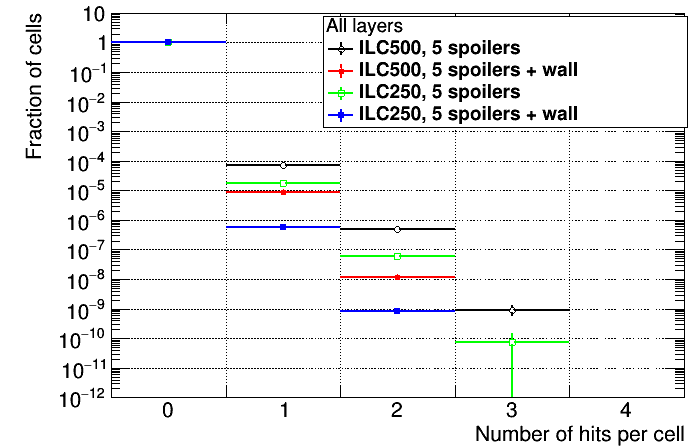
\includegraphics[width=\textwidth]{Figures/BDS_muons/Occupancy_Comparison_All_layers_wrt_cells_HcalBarrel.png}
   \caption{Normalized occupancy}
   \end{subfigure}
   \hfill
    \begin{subfigure}[b]{0.49\textwidth}
   \centering
    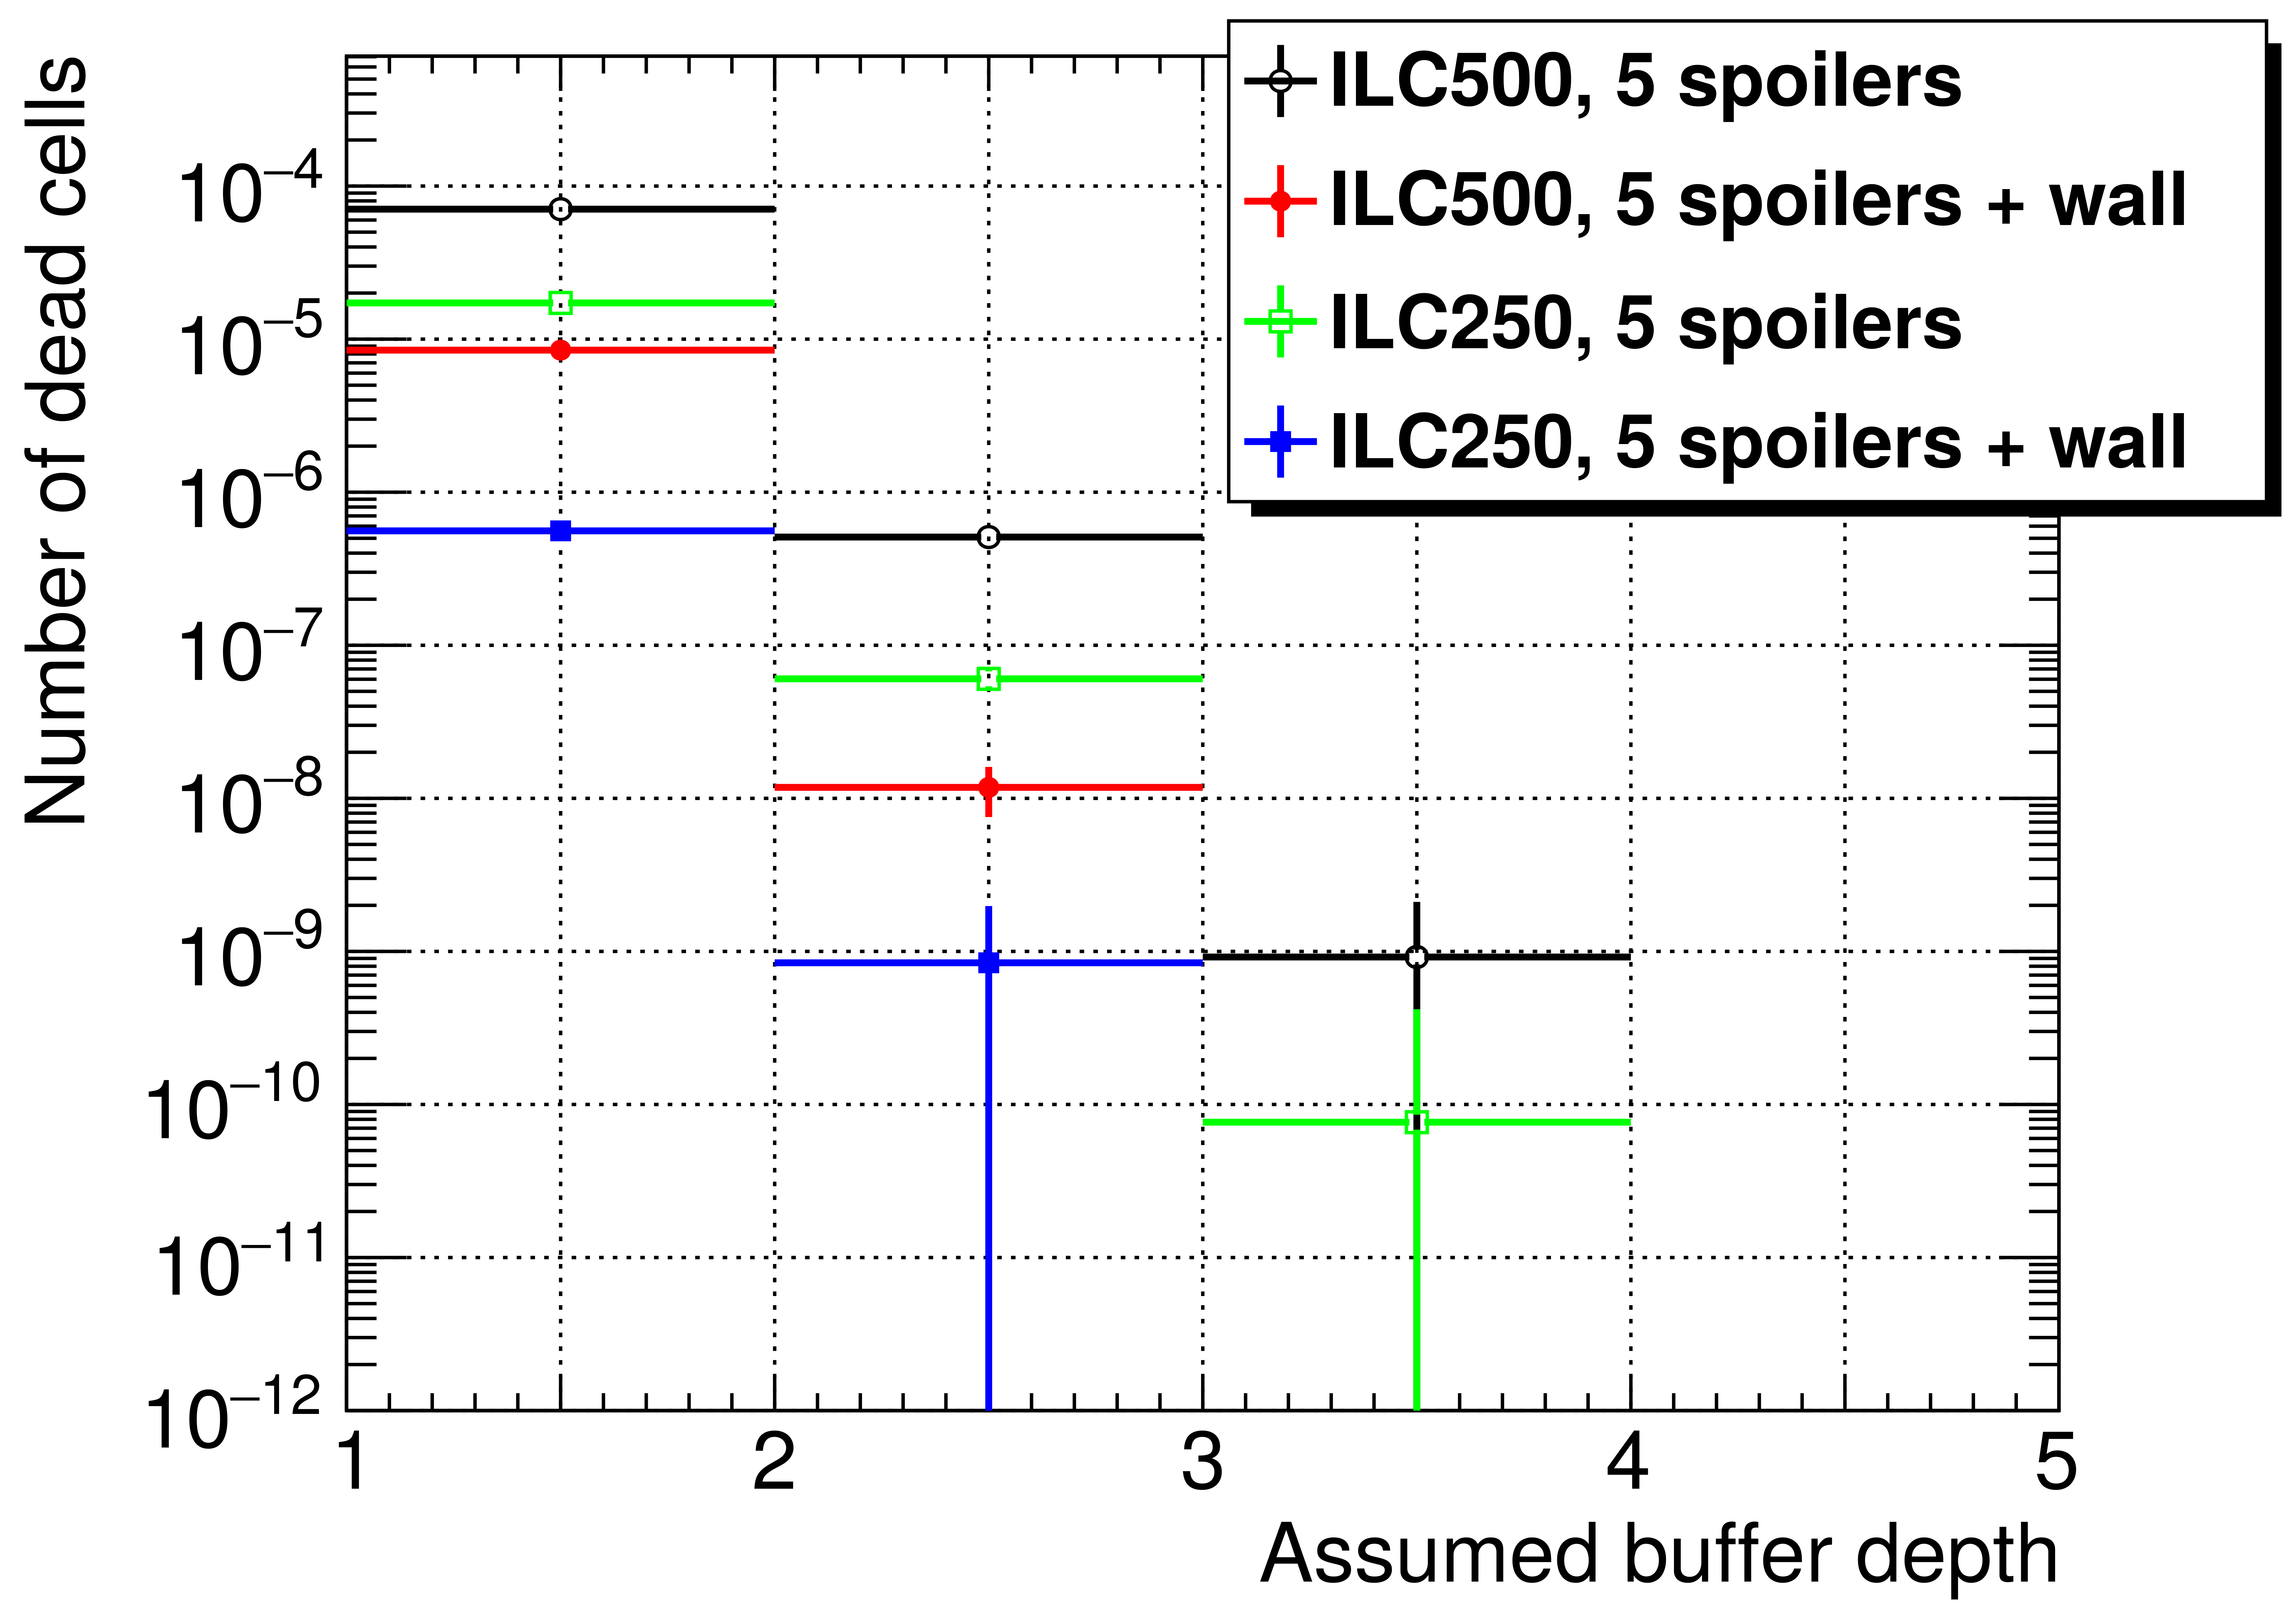
\includegraphics[width=\textwidth]{Figures/BDS_muons/Occupancy_Comparison_All_layers_deadcells_HcalBarrel.png}
   \caption{Normalized number of dead cells}
   \end{subfigure}
   \caption[SiD HCAL barrel occupancy from BDS muons]{Subfigure (a) shows the muon occupancy in the SiD HCAL barrel after a full bunch train, whilst subfigure (b) shows the number of dead cells resulting from this occupancy.
   Both histograms are normalized by the total number of cells in the HCAL barrel.
   The first bin of subfigure (a) contains the total number of cells, because of which the value of this bin is 1 for all cases.}
   \label{fig:BDS_Muons:HcalBarrel}
 \end{figure}
\\For the SiD tracker endcaps, however, the number of hits per cell reaches a maximum of 30 (see Figure~\ref{fig:BDS_Muons:SiTrackerEndcap}).
As the SiD tracker has a cell size of \SI{50}{\micro\meter}\,x\,\SI{50}{\micro\meter} in the current design, this is at first not to be expected.
The total number of hits in the tracker is smaller than in the HCAL, and yet the number of hits per cell reaches a much larger value.
The reason for this is that low energy (of the order of several hundred MeV) muons spiral in the magnetic field of the detector solenoid magnet, and by doing so hit the active layer of the tracker endcap several times.
An example of a loop performed by such a muon is depicted in Figure~\ref{fig:BDS_Muons:loop}.
Although the number of hits per cell ranges up to 30, the occupancy is consistently below \num{e-6} for all cases.
The number of dead cells, shown in Figure~\ref{fig:BDS_Muons:SiTrackerEndcap} (b), is plotted as a function of an assumed buffer depth of up to 30 accordingly.
Assuming the sensors in the SiD tracker will have a buffer depth of four, about \num{2e-8} of all cells would be dead for the ILC500 with the ``5 spoilers'' shielding only.
Also in this subdetector, the muon occupancy is below the critical limit for SiD for any buffer depth that might be chosen as the sensor design.
\\In the ILC500 stage, the occupancy for all subdetectors is reduced by at least a factor of five when adding a magnetized wall to the muon shielding.
This factor is even higher in the ILC250 stage.
Plots of the occupancy for the remaining SiD subdetectors can be found in Appendix~\ref{Appendix:BDS_Muons}.
  \begin{figure}
 \centering
  \begin{subfigure}[b]{0.49\textwidth}
   \centering
    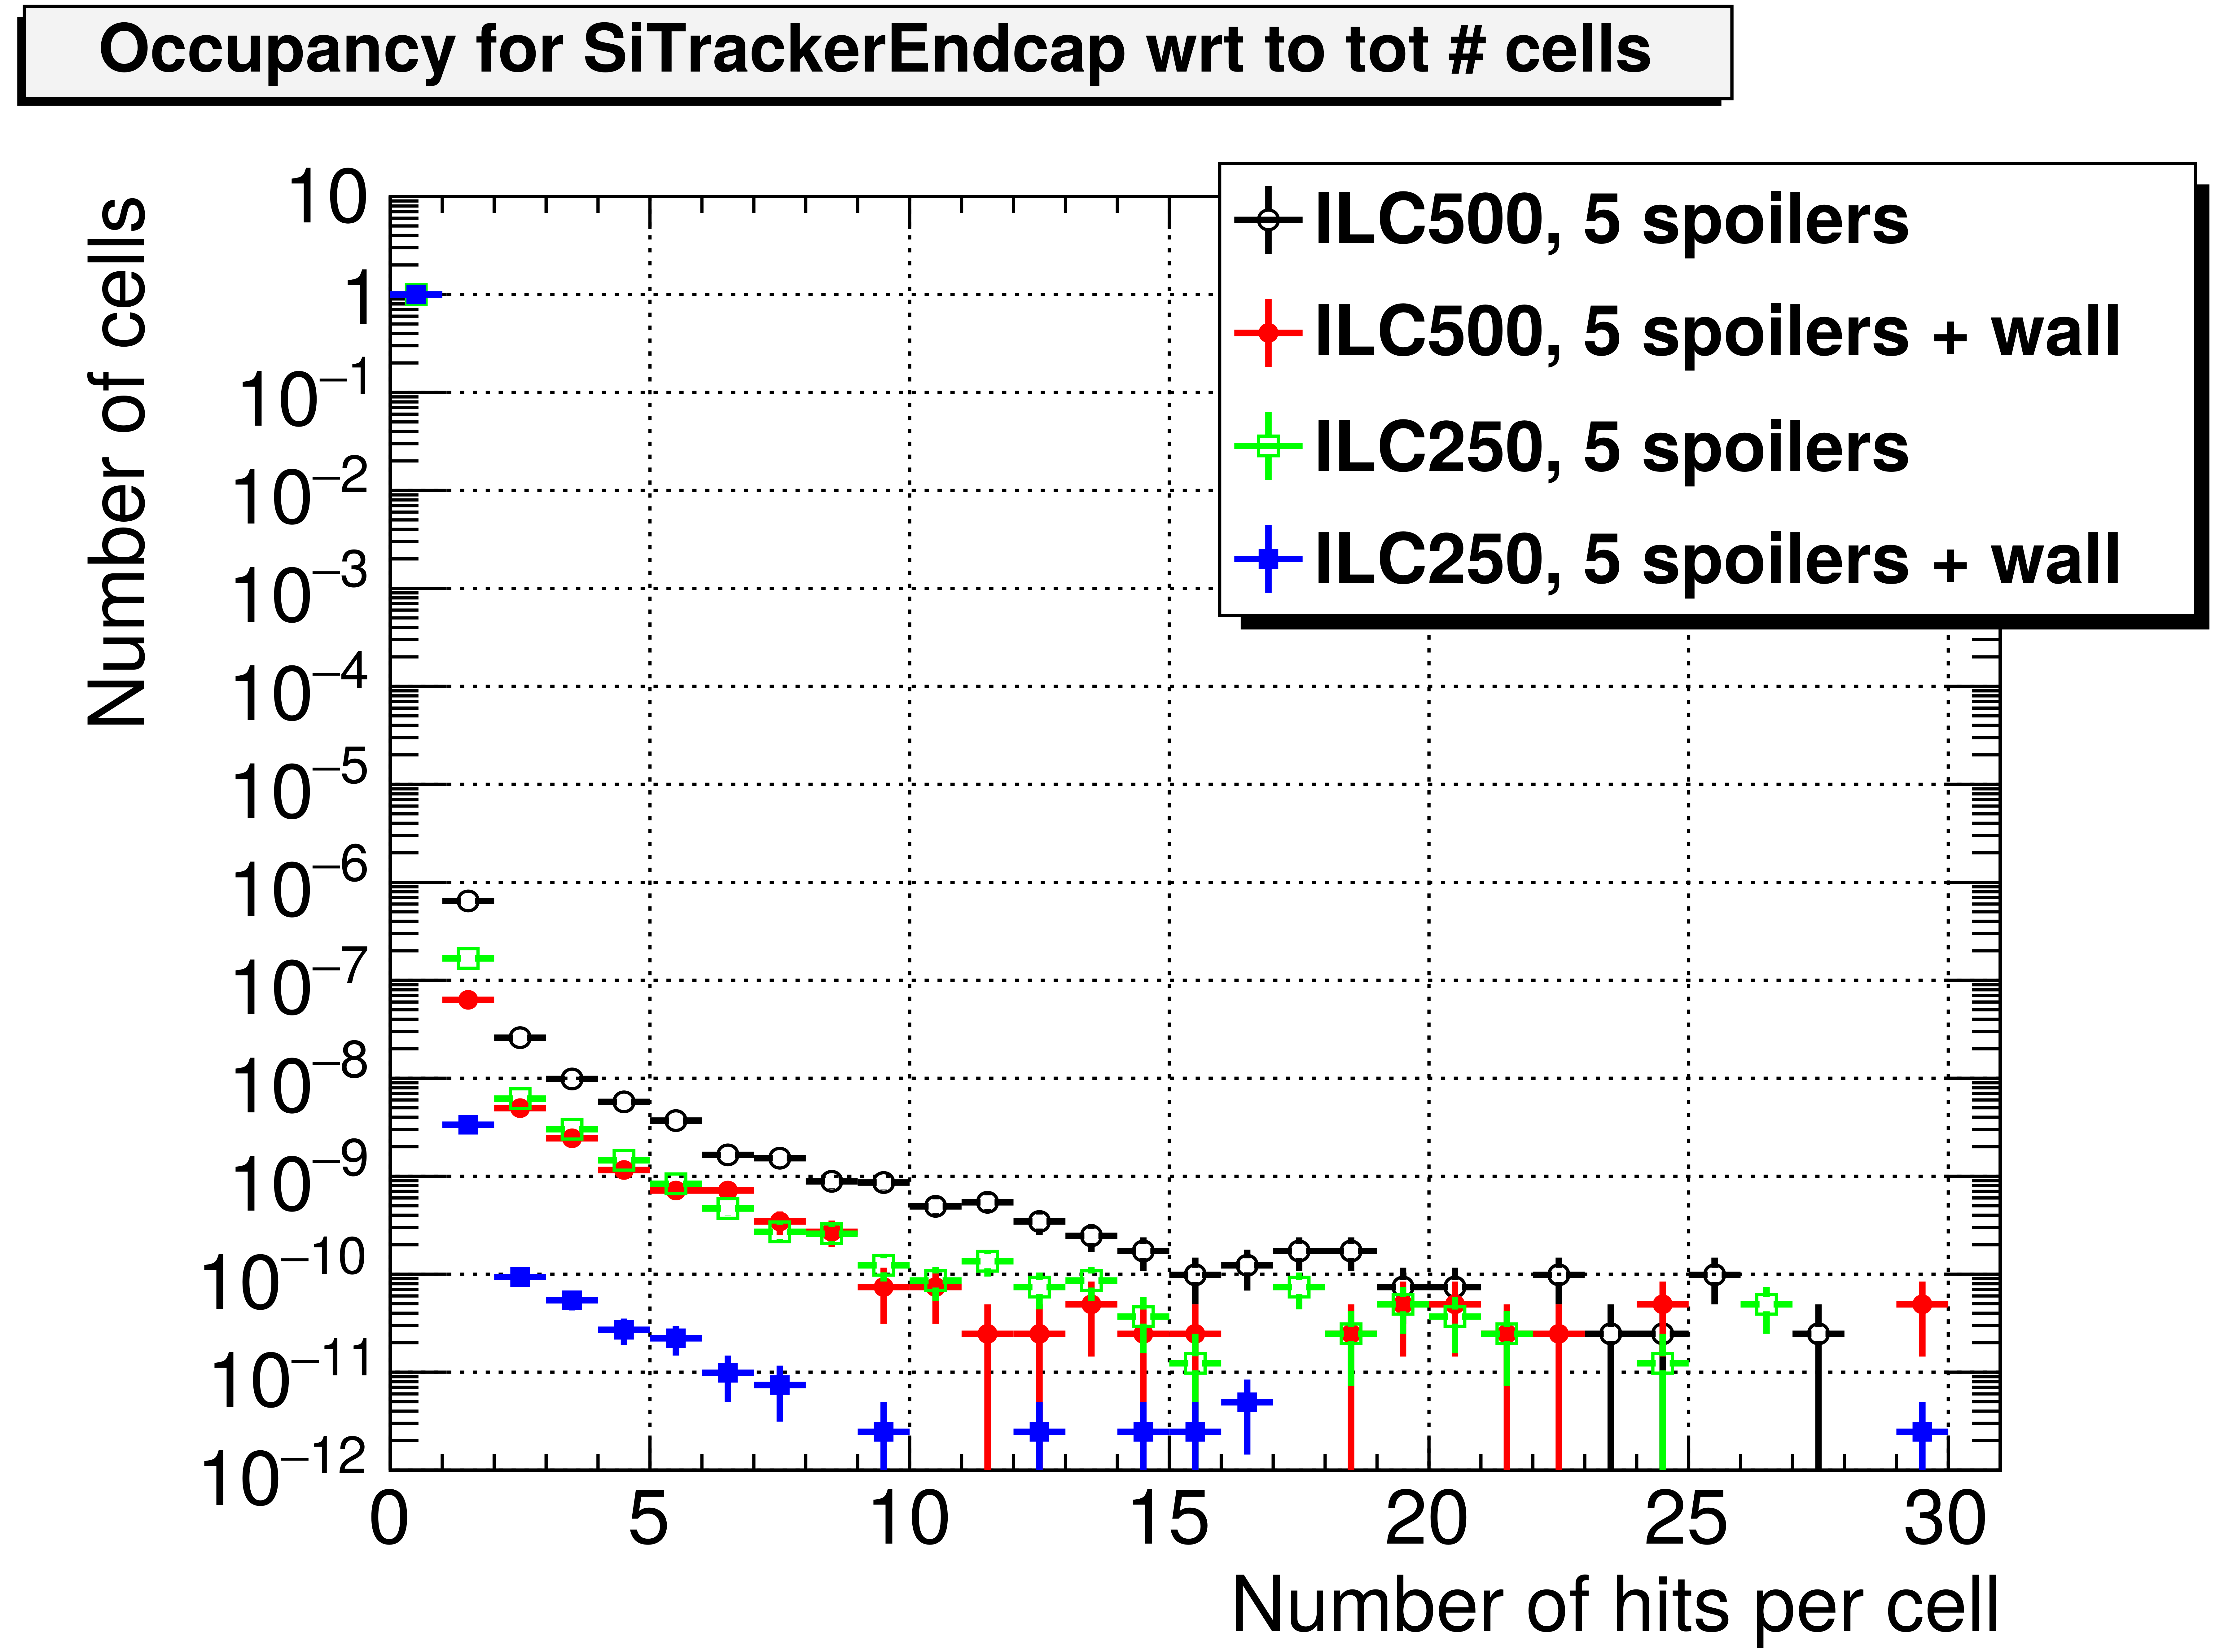
\includegraphics[width=\textwidth]{Figures/BDS_muons/Occupancy_Comparison_All_layers_wrt_cells_SiTrackerEndcap.png}
   \caption{Normalized occupancy}
   \end{subfigure}
   \hfill
    \begin{subfigure}[b]{0.49\textwidth}
   \centering
    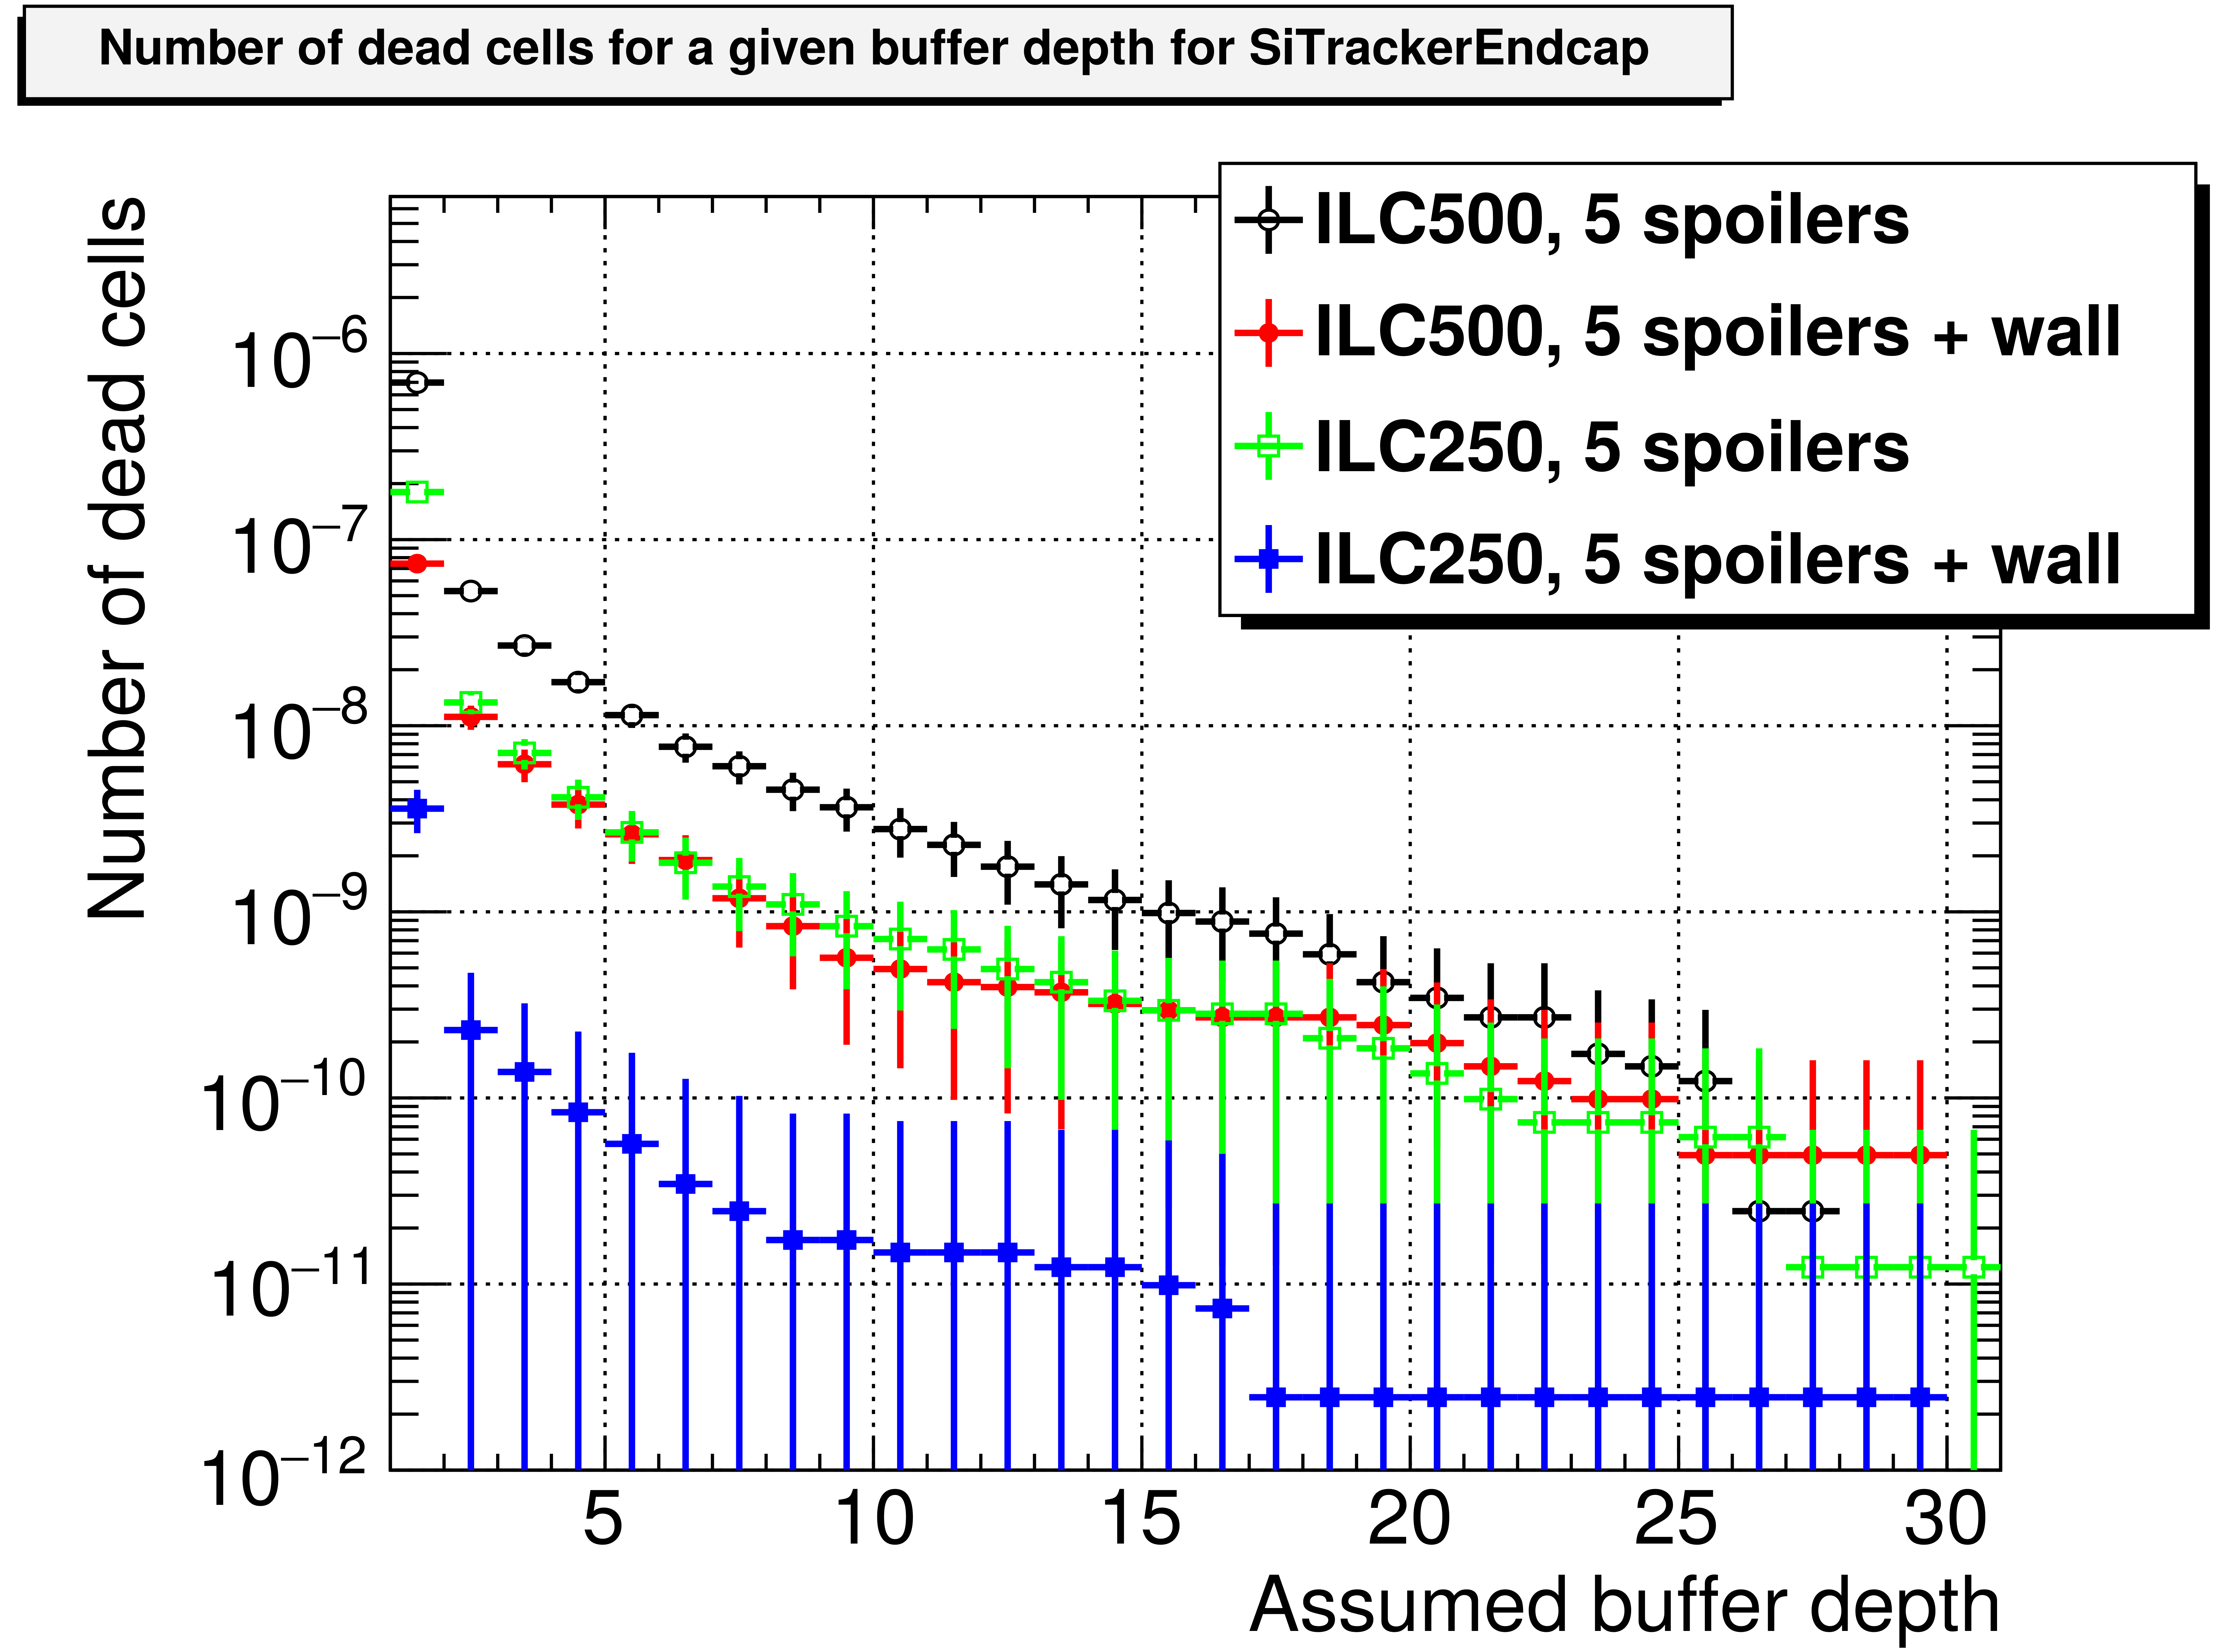
\includegraphics[width=\textwidth]{Figures/BDS_muons/Occupancy_Comparison_All_layers_deadcells_SiTrackerEndcap.png}
   \caption{Normalized number of dead cells}
   \end{subfigure}
   \caption[SiD tracker endcap occupancy from BDS muons]{Subfigure (a) shows the muon occupancy in one of the SiD tracker endcaps after a full bunch train, whilst subfigure (b) shows the number of dead cells resulting from this occupancy.
   Both histograms are normalized by the total number of cells in the tracker endcap.
   The first bin of subfigure (a) contains the total number of cells, because of which the value of this bin is 1 for all cases.}
   \label{fig:BDS_Muons:SiTrackerEndcap}
 \end{figure}
 
 \begin{figure}[htbp!]
\centering
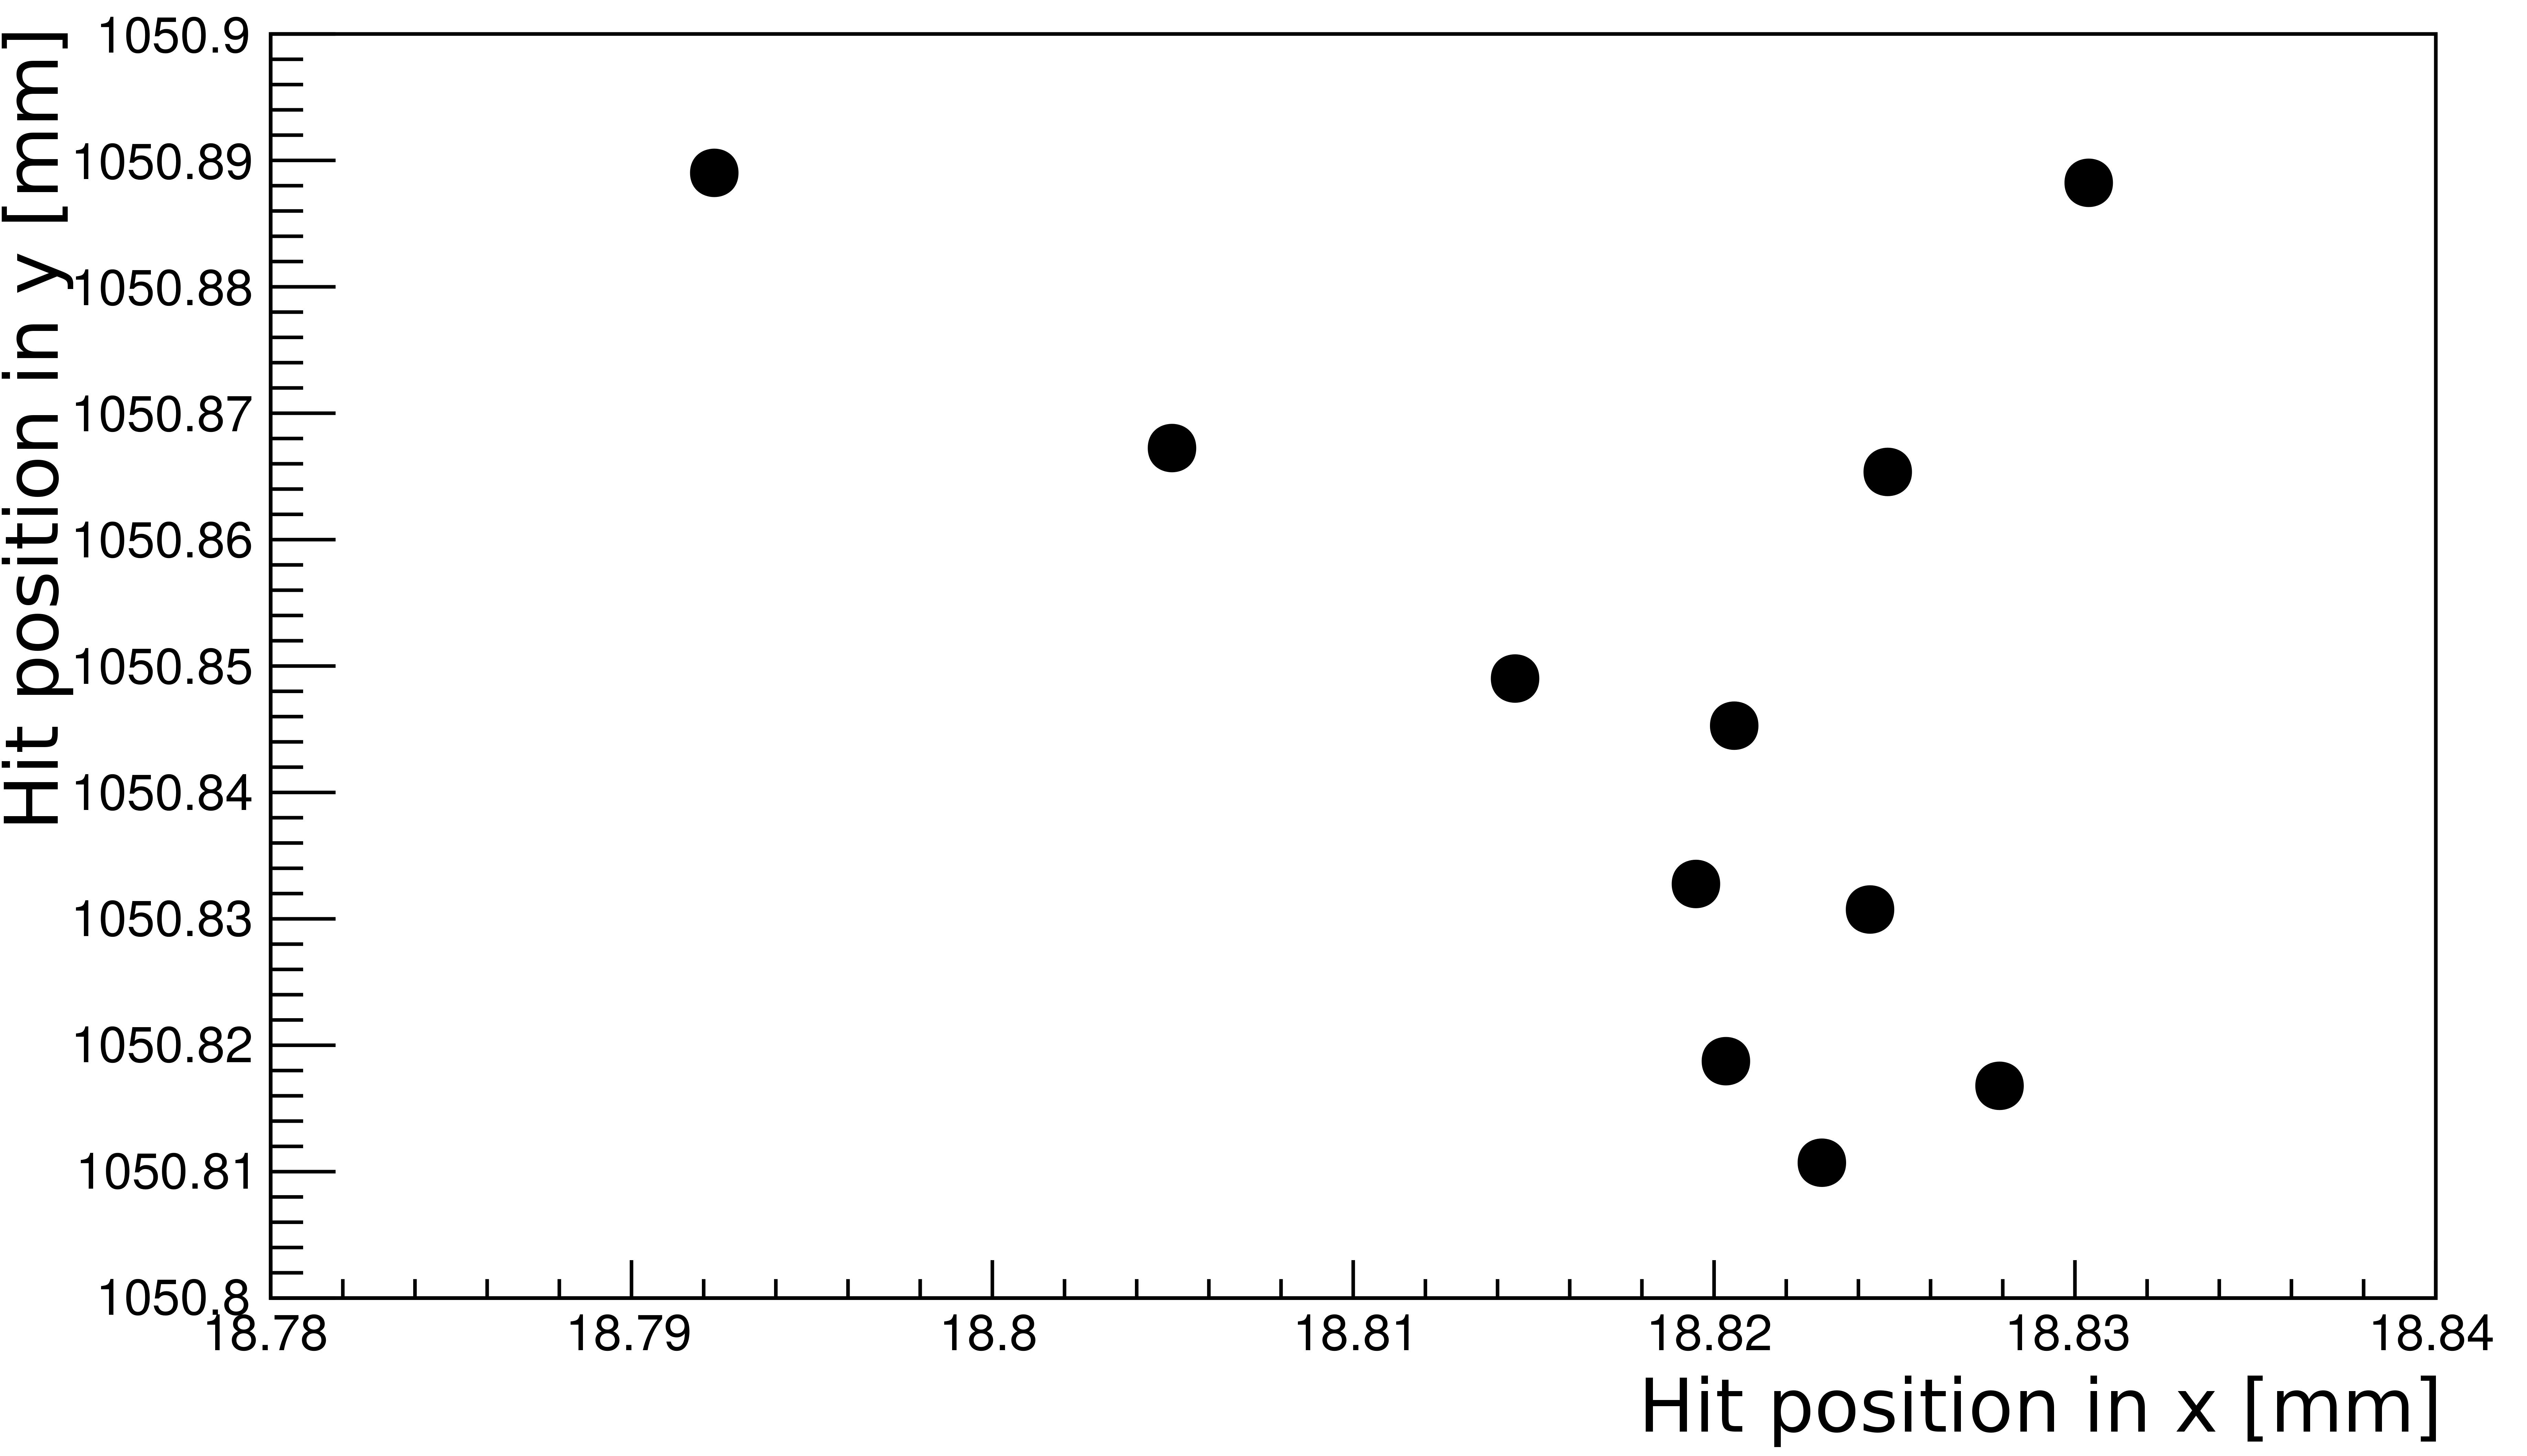
\includegraphics[width=0.5\textwidth]{Figures/BDS_muons/LoopInACell.png}
\caption[BDS muons looping]{Hit position of muon hits in the SiD tracker endcap, in layer number four.}
\label{fig:BDS_Muons:loop}
\end{figure}

\subsection{Conclusion}
This section presented a study of the effect of the muons from the BDS on the SiD occupancy for two different shielding options.
For the first option, five magnetized spoilers would be installed at different locations along the beam line.
For the second option, a magnetized wall would be placed between these spoiler locations and the interaction region, as an additional shielding device.
The comparison of the occupancy in these two cases revealed that the magnetized wall reduces the occupancy by a significant amount.
Nevertheless, the occupancy level is in both cases far from the critical limit of \num{e-4}, which is especially important in the tracking systems of the SiD detector.
For these subdetectors, a minimal background occupancy is crucial to guarantee a high performance in the track reconstruction of physics events.
For a center-of-mass energy of \SI{250}{\GeV} in the first ILC stage, the SiD tracker endcap occupancy for an assumed buffer depth of four is about \num{4e-9} for the minimal shielding option without the wall.
Since in the next ILC stage at a center-of-mass energy of \SI{500}{\GeV}, the number of muons reaching the detector is larger by a factor of three, also the occupancy for the same buffer depth is increased by about a factor of three for the ``5 spoilers'' case.
However, it still does not exceed \num{e-7}.
\\Overall, the magnetized wall does not seem to be necessary in order to limit the muon occupancy in SiD, for both studied center-of-mass energies.
However, the wall serves as a tertiary containment device against muons and other machine background particles.
The decision might be to keep the wall anyway for the protection of personnel and maintenance staff, depending on the law restrictions.
A solution to lessen the price for the wall would be to change its design such that its thickness is reduced and it is not magnetized.
The wall would then still serve as additional shielding but does not deflect charged particles. \\An idea for future studies of the muon shielding would be to also adjust the detector specific Pacman design with respect to different materials and the possibility of magnetizing the Pacman volume.

%---------------------------------------------------
\section{Background from beam halo collimators in the final-focus system}

The Final-Focus System (FF) is -as explained in Chapter~\ref{ILC}- responsible for focussing the beam to nanometre size. The reason behind this is the need for high luminosities which can be gained by small beam sizes. Another goal of the International Linear Collider is to have clean events with as little background as possible. A solution to this is to install beam halo collimators in the FF system that cut off the halo around the beam core. As the beam halo can interact with the beam pipe and its components, a beam halo collimation system plays an important role in the reduction of background at the IP. Nevertheless, the collimator itself can be source to particle showers and rises in the background level around the collimator location. Feasibility studies are needed to investigate in the effect of a beam halo collimator.\\
A vertical beam halo collimator was installed at the Accelerator Test Facility 2 (ATF2) at the research centre KEK in Japan. In March 2016, data of the background was taken with a Cherenkov detector in dependency of the aperture of this collimator at ATF2. This section covers the analysis of the data as well as the comparison of the data with simulations done with \bdsim. Both, the design of the vertical beam halo collimator at ATF2 and the \geant simulation tool \bdsim are explained here additionally.

\subsection{Beam halo collimator}
\label{Collimator}

The vertical beam halo collimator, for which the design drawings are shown in Figure~\ref{fig:collimator}, was installed in ATF2 in the beginning of March 2016. The collimating jaws are inside a structure that is evacuated and connected to the beam pipe of the ATF2 beam line. The actual jaws are made of Copper, the rest of the components in the collimator structure are out of Stainless Steel. The jaws have a width of ?? and thickness of ??.
%TODO: Add information about measurements of the jaws and the whole structure

\begin{figure}
\centering
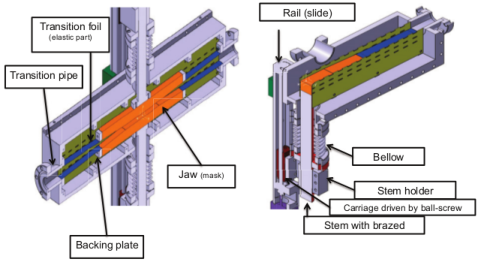
\includegraphics[width=0.8\textwidth]{Figures/ATF/ATF2_beamhalo_collimator.pdf}
\caption[Drawing of the beam halo collimator]{A drawing of the vertical beam halo collimator built into ATF2.\cite{NuriaCollimator2015}}
\label{fig:collimator}
\end{figure}

The two jaws can be moved individually to an arbitrary position, so that the edge of the jaw has a distance of between 2.6 and \SI{12}{\milli\metre} with respect to the centre. Therefore, the full aperture of the collimator structure can be between 5.2 and \SI{24}{\milli\metre}. The error on the position of the jaws is about \SI{0.04}{\milli\metre}.\\
As every component in a beam line, especially for such small beam sizes, is affecting the electromagnetic field of the passing beam, the collimator is designed to minimize the effect of inducing large wakefield. The concern of wakefields induced by the collimator is addressed in \cite{NuriaCollimator2015}. This thesis chapter focusses exclusively on the effect on the background level.

\begin{figure}
\centering
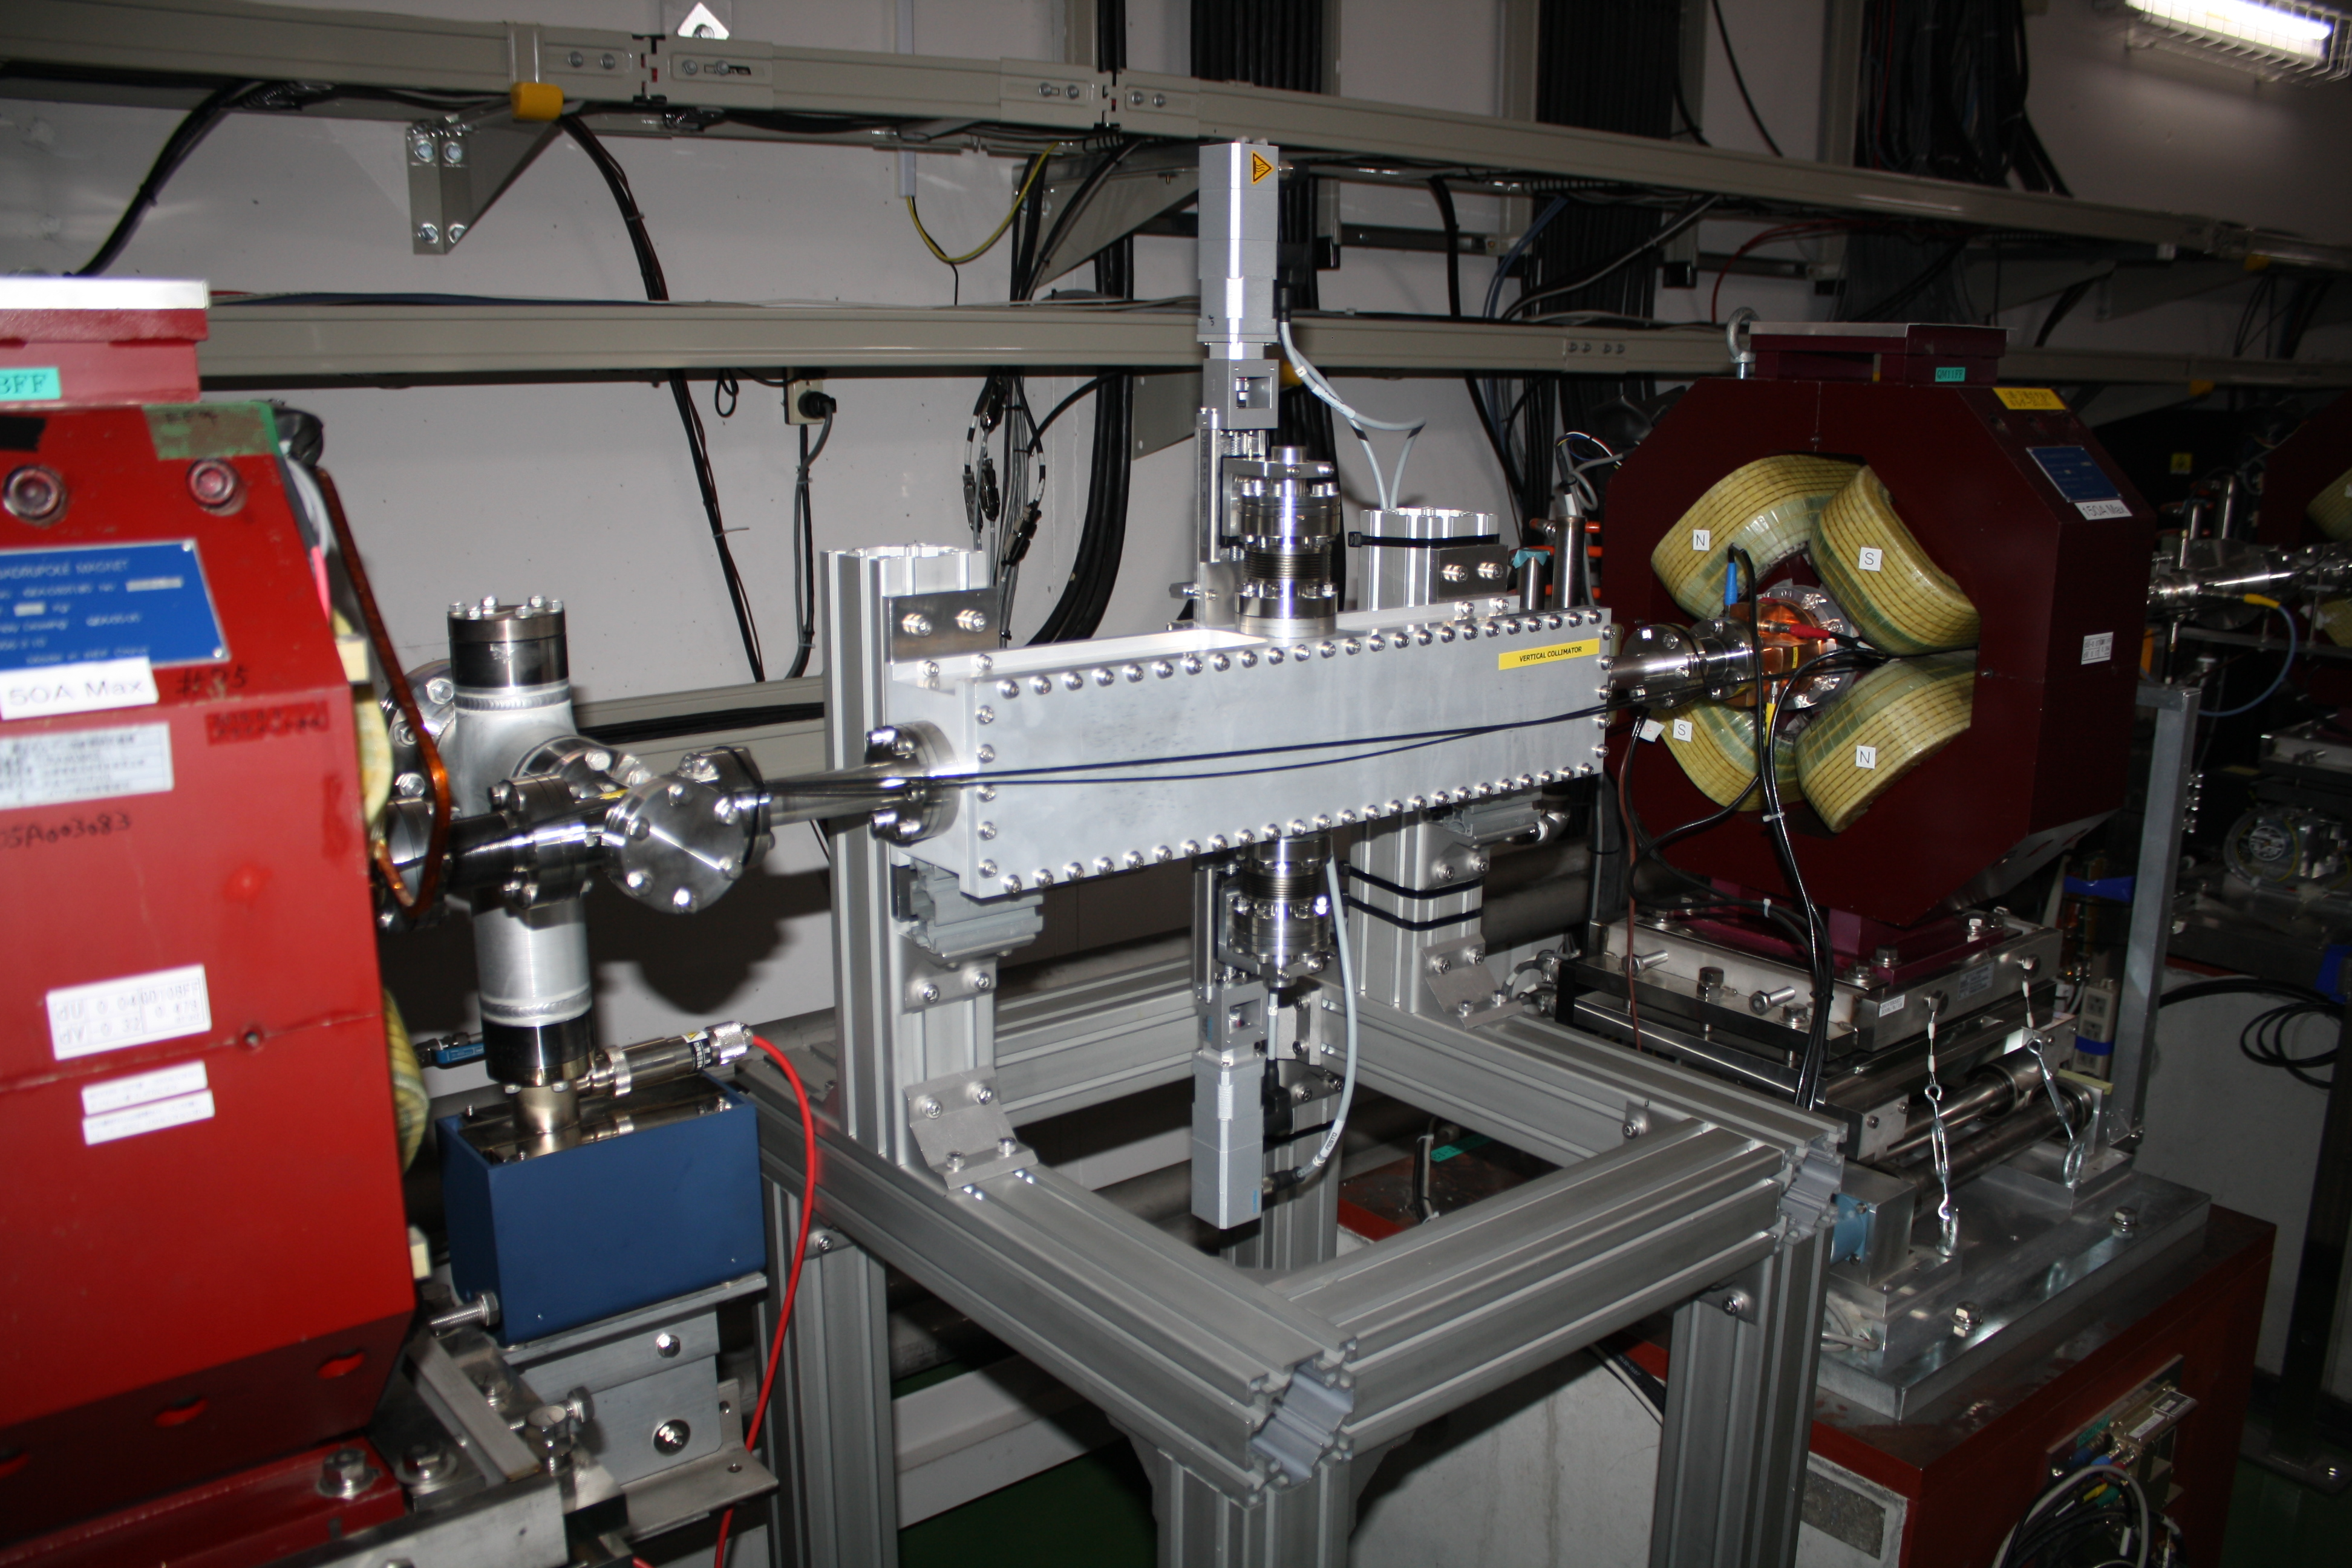
\includegraphics[width=0.8\textwidth]{Figures/ATF/Installed_Collimator.jpg}
\caption[Picture of the installed beam halo collimator]{A picture of the vertical beam halo collimator built into ATF2. The collimator jaws are within the evacuated structure. At the top and bottom of the structure, you can see the mover system for the two jaws.}
\label{fig:installed_collimator}
\end{figure}

\subsection{The Accelerator Test Facility 2}
\label{ATF2}

The Accelerator Test Facility 2 (ATF2) is an extension to the accelerator facility ATF at the research centre KEK in Japan. As can be seen in Figure~\ref{fig:ATF}, ATF consists of a linear accelerator which pre-accelerates the particles before they are accessing the dumping ring. Before the ATF2 was built, the beams were dumped after leaving the dumping ring through the short extraction line.\\ATF2 is a test bench for the FF system of the ILC and has two main goals: Focussing the low-emittance beam to \SI{37}{\nano\metre} in the vertical plane, and demonstrating the stability of the nanometre sized beam at the interaction point. So far a repeatable beam size of \SI{40}{\nano\metre} has been shown. Although the beam size goal of ATF2 seems to be too large compared to the ILC goal of \SI{9}{\nano\metre}, the ATF2 system is very close to the ILC FF. The beam size goal has to be scaled up for different lattice and beam conditions.

\begin{figure}
\centering
\includegraphics[width=0.6\textwidth]{Figures/ATF/ATF.jpg}
\caption[ATF accelerator]{A schematic of the ATF accelerator with the ATF2 extension. The ATF consists of a linear accelerator, a beam dump, the old extraction line, and the new ATF2 extension.}%TODO: cite the source of the ATF figure!
\label{fig:ATF}
\end{figure}

The vertical beam halo collimator and the Cherenkov detector, with which the background level in dependency of the collimator aperture was measured, are both located in the Final-Focus region of ATF2. The location of the collimator was chosen in such a way that the phase of the beta function is the same as at the IP. Due to that the effect of the collimation of the beam halo is then visible at the IP as desired. A schematic of the ATF2 lattice with the beam halo collimator and the Cherenkov detector is shown in Figure~\ref{fig:ATF2}. The Cherenkov detector was built and setup by a group of the Royal Holloway University of London (RHUL) because of which the detector is in the following referred to as the 'RHUL Cherenkov detector'. A more detailed description of this detector is given in Section~\ref{RHUL}.

\begin{figure}
\centering
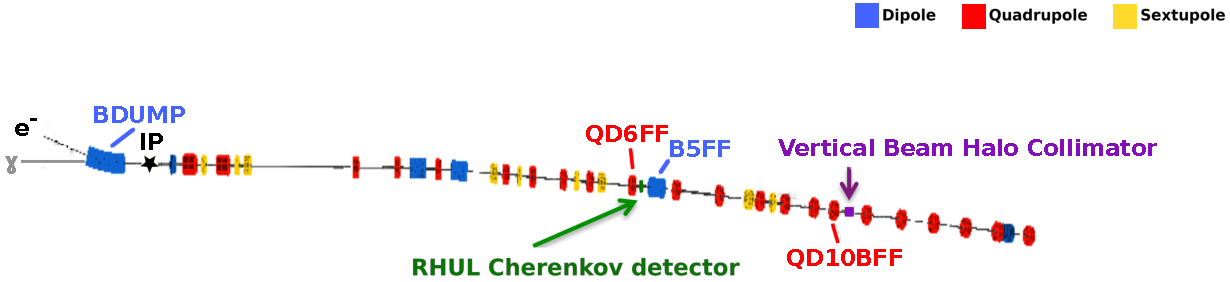
\includegraphics[width=\textwidth]{Figures/ATF/ATF2schematic.pdf}
\caption[ATF2]{A schematic of the ATF2 lattice. The beam direction is from right to left. The different magnets of the lattice are colour schemed: the bending dipole magnets are coloured in blue, the quadrupoles in red, and the sextupoles in yellow. The beam halo collimator is located before the quadrupole magnet 'QD10BFF', and the Cherenkov detector downstream between the dipole magnet 'B5FF' and the quadrupole magnet 'QD6FF'. After the interaction point (IP), the electron beam is bend in the last dipole magnet 'BDUMP' towards the beam dump. The neutral particles, like the photons, are continuing in a straight line where they can be monitored by the IPBSM Background Monitor. The Diamond Sensor (DS) can measure the shape of the beam core and the halo, before the beam is dumped.}
\label{fig:ATF2}
\end{figure}

\subsection{BDSIM}
\label{BDSIM}
\bdsim is a \geant extension toolkit for simulation of particle transport in accelerator beamlines. It was developed and is still supported by RHUL.
The geometry of lattice parts are described in classes within the \bdsim framework. Lattices, like the ATF2 lattice, can easily be built up by the pre-defined components. A figure of the ATF2 lattice visualized with the \bdsim software is shown in Figure~\ref{fig:ATF2_BDSIM}.
\begin{figure}
\centering
\includegraphics[width=0.7\textwidth]{Figures/ATF/atf_bdsim.png} %TODO: exchange with a recent one of ATF2
\caption[ATF2 lattice in \bdsim]{A part of the ATF2 lattice visualized with the \geant toolkit \bdsim.}
\label{fig:ATF2_BDSIM}
\end{figure}
Accelerator descriptions from other tools such as MADX can be converted to \bdsim input. 

\begin{itemize}
 \item BDSIM framework at DESY - explain
\end{itemize}

%---------------------------------------------------
\subsection{Background studies}
\subsubsection{RHUL Cherenkov detector}
\label{RHUL}

The RHUL Cherenkov detector was built by a group from the Royal Holloway University of London. It uses the Hamamatsu PMT, which was used for a laserwire sensor that was located at the same position before. The Cherenkov detector itself is using aerogel\footnote{SP15, index 1.015, 4 slices, 4 cm$^2$, 5 cm deep}. A light pipe, with a profile area of \SI{10}{\centi\metre\square} and a total length of \SI{35}{\centi\metre}, directs the light from the aerogel to the PMT.

\begin{figure}
\centering
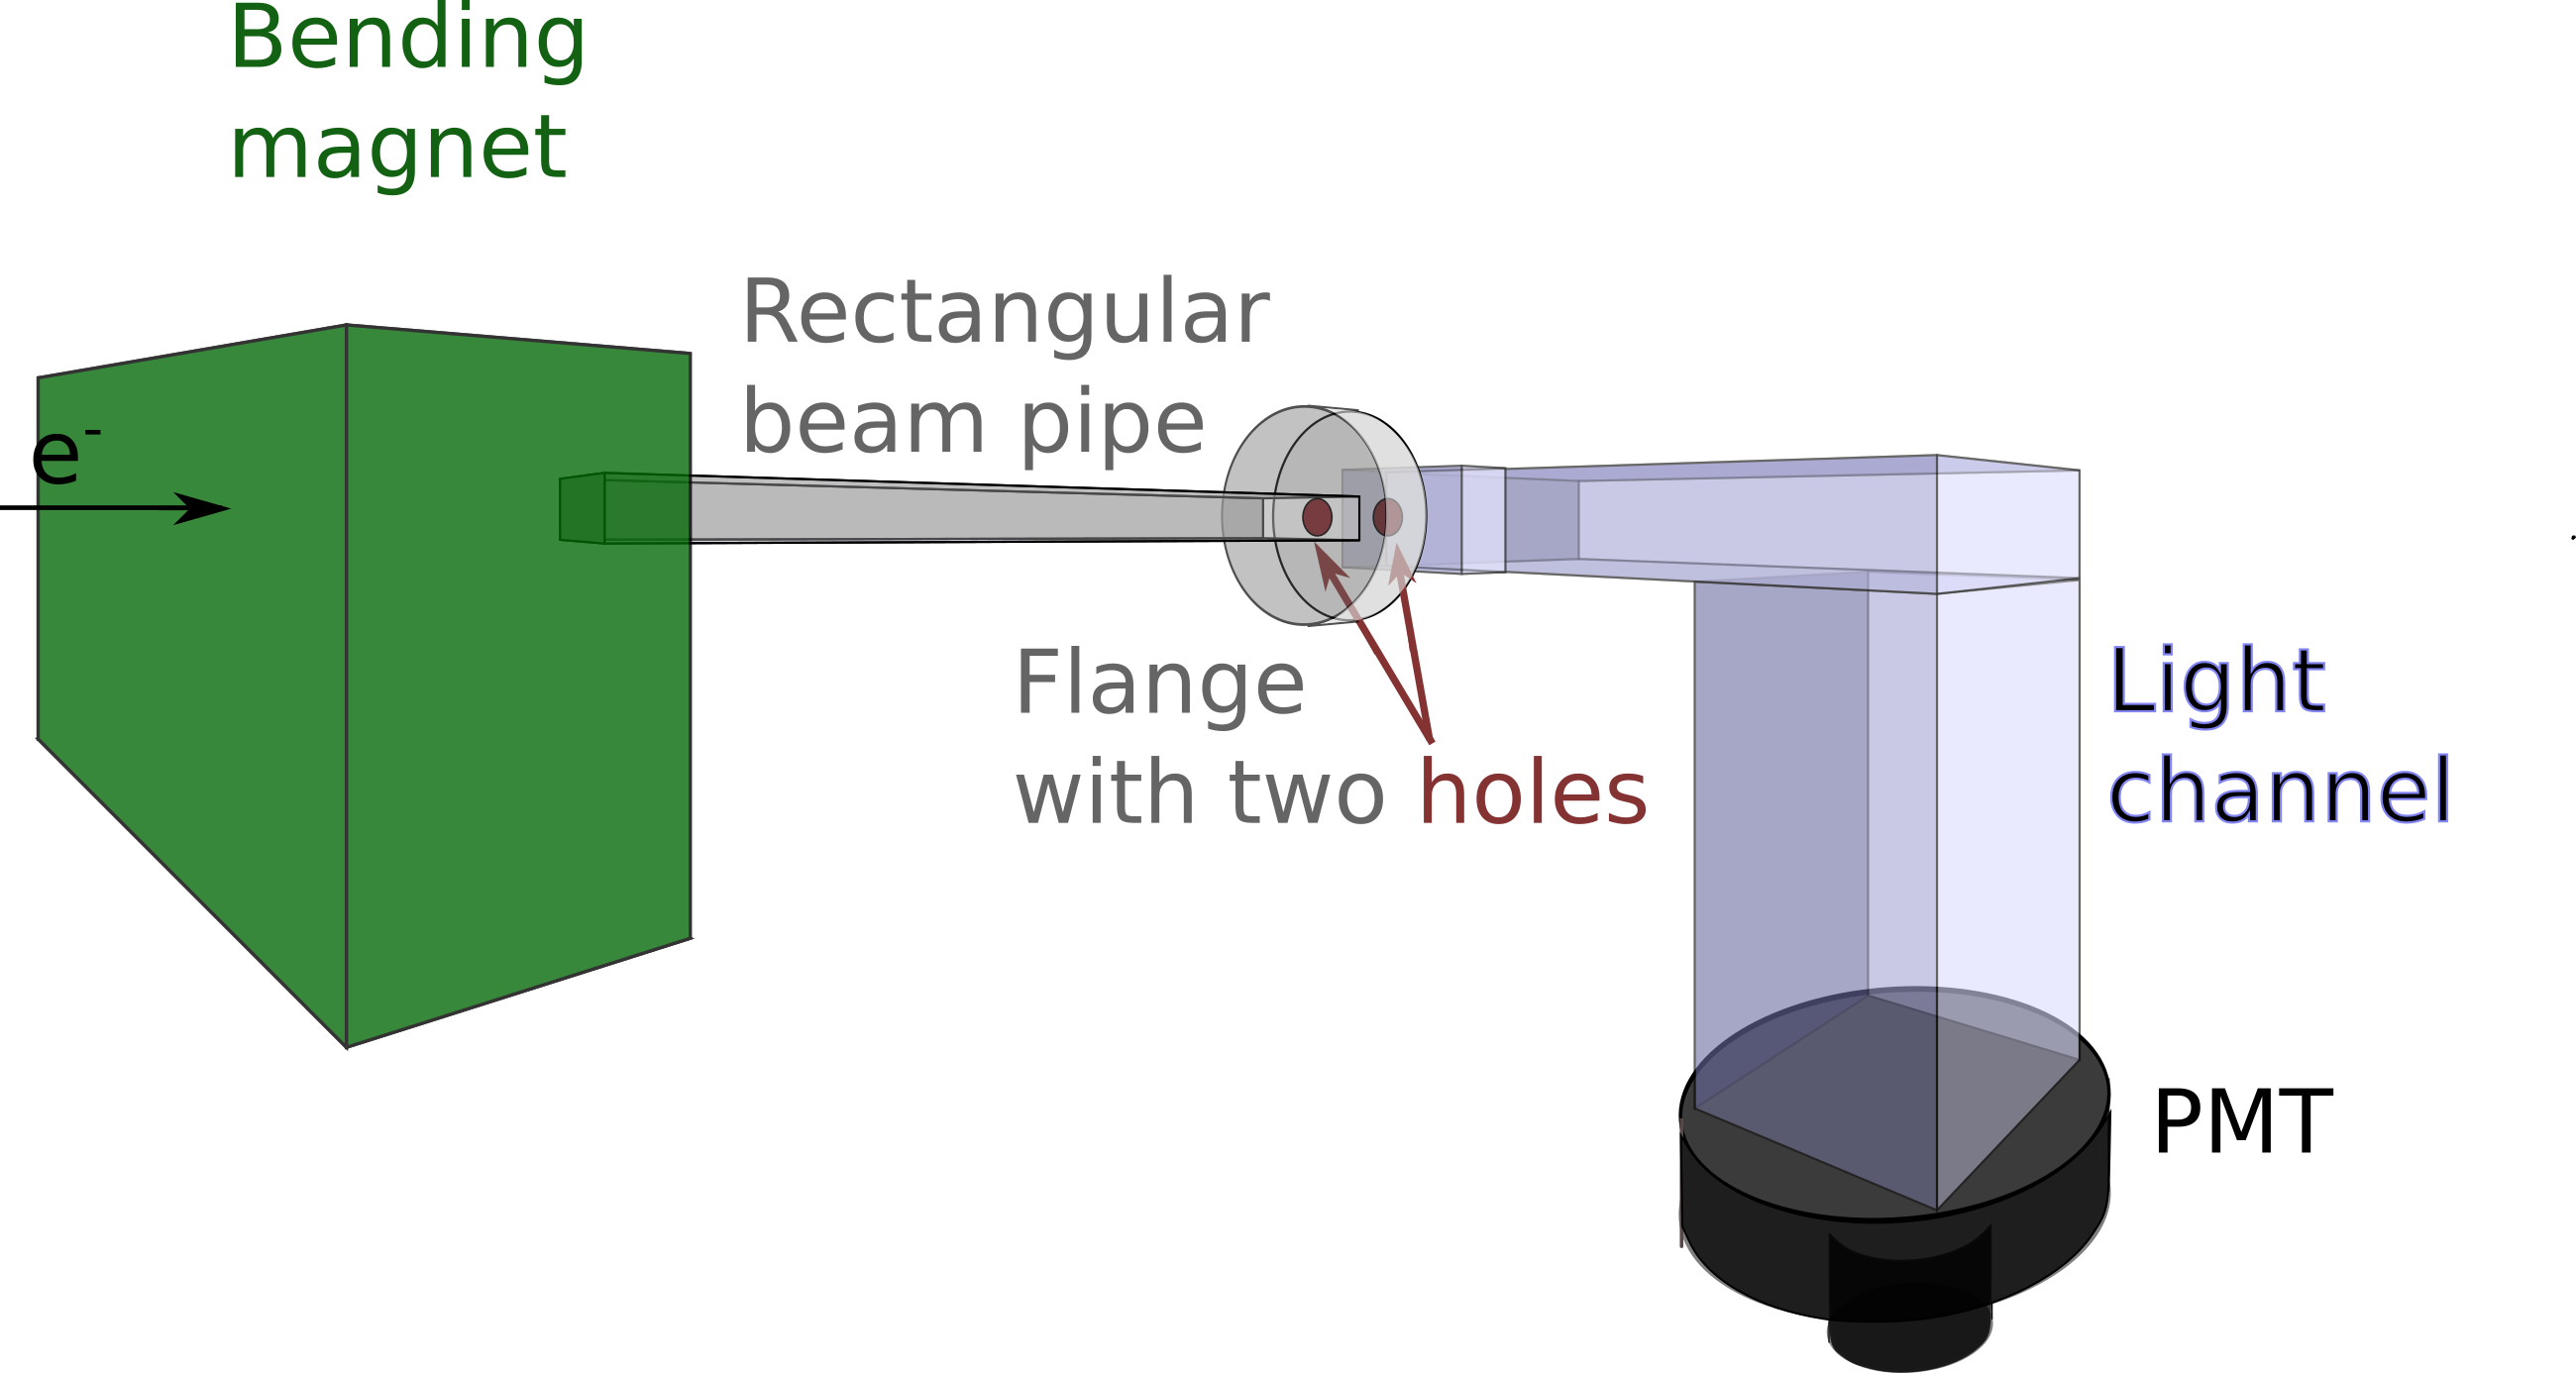
\includegraphics[width=0.8\textwidth]{Figures/ATF/drawing_CherenkovSetup.png}
\caption[Schematic drawing of the RHUL Cherenkov detector setup]{A perspective schematic of the RHUL Cherenkov detector setup in ATF2. The electrons of the beam core are bent in the dipole magnet, and continue through the rectangular and circular beam pipes along the ATF2 beam line. The neutral particles on the other hand, which are not deflected in the magnetic field, are continuing on a straight line through the rectangular beam pipe, and enter the RHUL Cherenkov detector through the second window in the flange. The light signals are collected by the PMT.}
\label{fig:RHUL_Cherenkov_Drawing}
\end{figure}

\begin{figure}
\begin{center}
\resizebox{.9\textwidth}{!}{%
\includegraphics[height=0.35\textheight]{Figures/ATF/CherenkovDetector_inBeamLine1.jpg}%
\quad
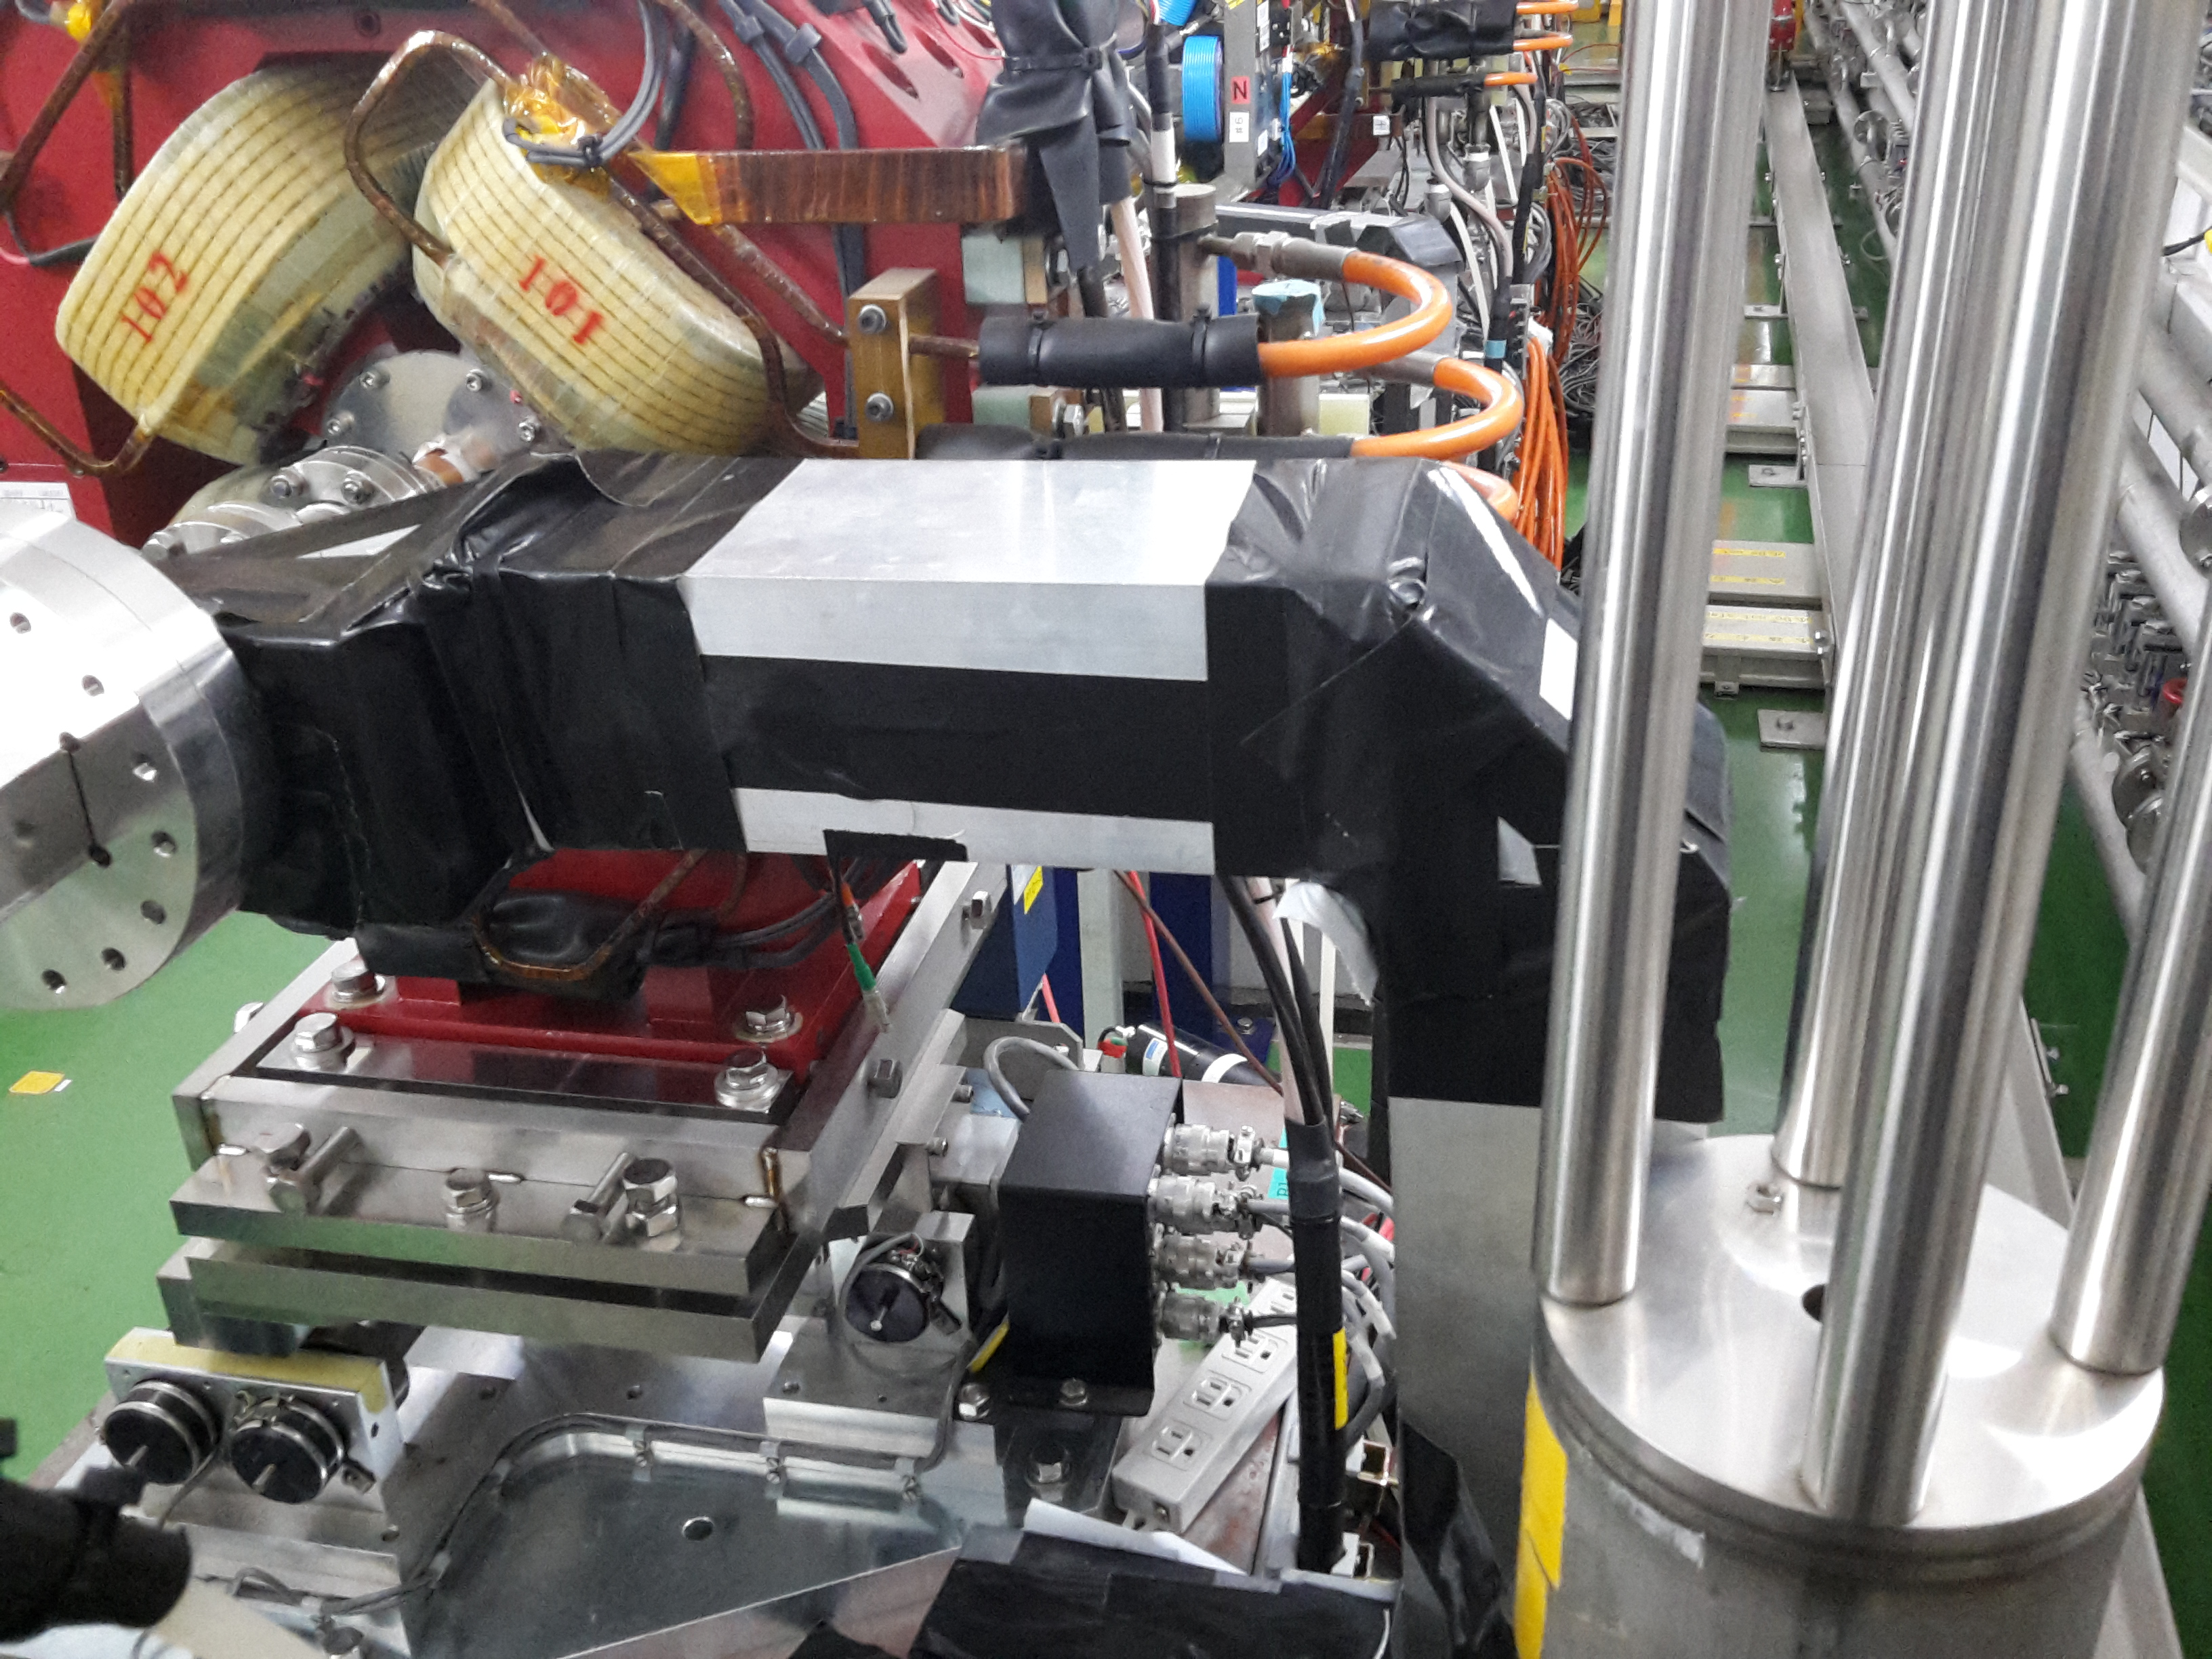
\includegraphics[height=0.35\textheight]{Figures/ATF/CherenkovDetector_inBeamLine2.jpg}%
}
\caption[Pictures of the RHUL Cherenkov detector]{Pictures of the RHUL Cherenkov detector in ATF2. The aerogel detector and the light channel is positioned behind a flange that connects a rectangular beam pipe with a circular one. The flange has two openings, one for the circular beam pipe, another one covered by a plastic window through which the photons leave the rectangular beam pipe and enter the RHUL Cherencov detector.}
\label{fig:RHUL_Cherenkov}
\end{center}
\end{figure}

\paragraph{PMT noise measurements}
\begin{figure}
\centering
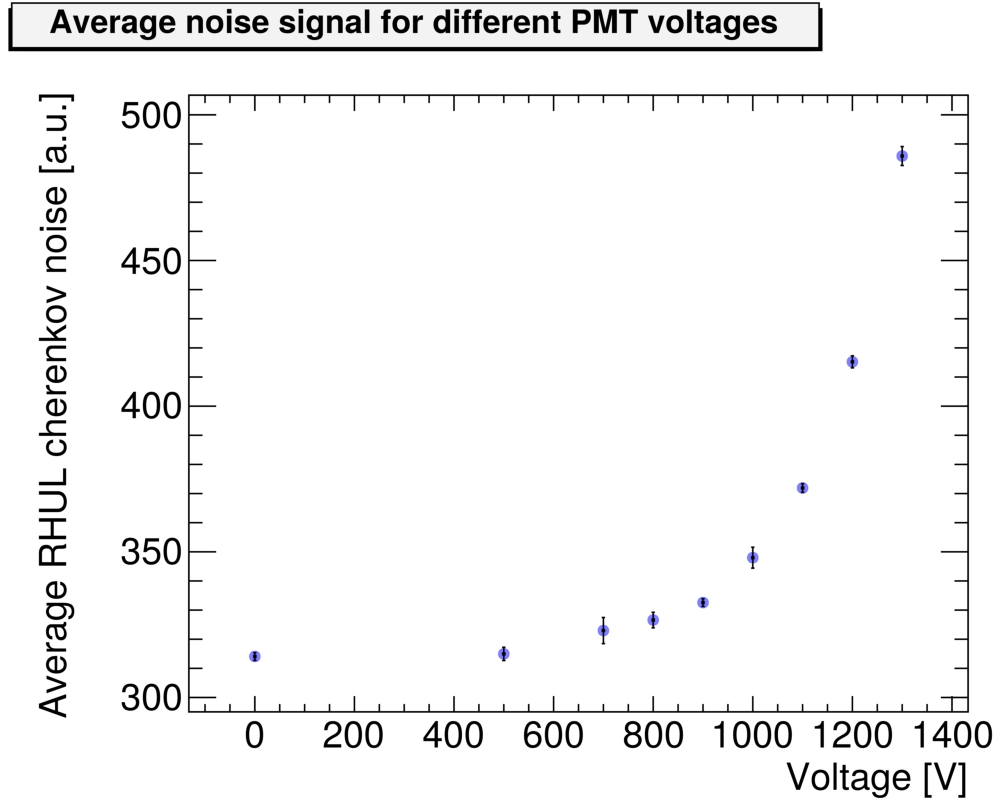
\includegraphics[width=\textwidth]{Figures/ATF/AverageNoise_perVoltage_08April.pdf}
\caption[RHUL Cherenkov detector noise]{Average PMT noise signal as a function of the voltage applied to the detector PMT. The noise was measured when the ATF beam was turned off. For each voltage, 500 or 1000 ADC pulses of noise were recorded, and the noise averaged over the number of pulses. The error bars to the mean values are the standard deviation of the mean.}
\label{fig:AverageNoise}
\end{figure}
Figure ~\ref{fig:AverageNoise} shows the mean values of the noise measurements for different PMT voltages. For every point either 500 or 1000 ADC pulses were recorded and averaged. The error bars represent the standard deviation on the mean value calculated by $SD=\frac{\sigma}{\sqrt{N}}$, where $\sigma$ is the RMS of the noise distribution at each point and N the number of pulses.\\
At around \SI{800}{\volt} the effect of dark current in the PMT starts getting prominent wherefore the noise rises exponentially. For the data shown in the following, the noise is already subtracted. As the data was taken only for these voltages, for which noise measurements were done, the mean value of noise is subtracted from every signal pulse appropriately. Therefore the rise in noise is automatically taken into account for higher voltages.

\paragraph{PMT voltage calibration measurements}
\begin{figure}
\centering
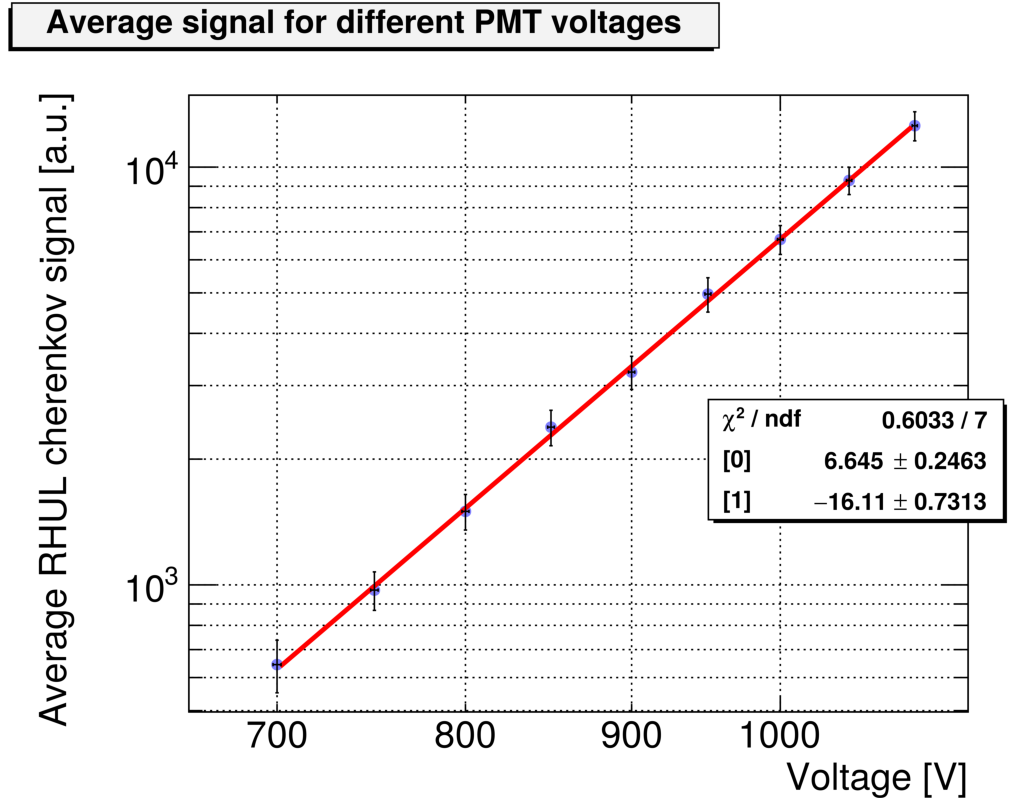
\includegraphics[width=\textwidth]{Figures/ATF/VoltageNormalization_totError.pdf}
\caption[RHUL Cherenkov detector voltage calibration]{Average PMT signal as a function of the voltage applied to the detector PMT. The signal was measured when the ATF beam was stable at a beam intensity of \num{0.15}$\pm$\num{0.02e10}. For each voltage, 500 ADC pulses were recorded, and the signal averaged over the number of pulses. The error bars to the mean values are the standard deviation of the signal distributions measured for each voltage.}
\label{fig:VoltageNormalization}
\end{figure}

In order to compare data sets that are taken at different PMT voltages, the signals have to be scaled. The rule of scaling the data is derived from the fit to the calibration measurements in Figure~\ref{fig:VoltageNormalization}. The data for this calibration is taken for stable beam conditions at a beam intensity of \num{0.15}$\pm$\num{0.02e10}, and then plotted in a log-log plot. The linearity of the data points show the behaviour of the PMT for different voltages according to Equation~\ref{eq:PMTgain}\cite{Hamamatsu}:
\begin{equation}
 \mu = A \cdot V^{kn} 
 \label{eq:PMTgain}
\end{equation}
where \textmu is the PMT gain, V the applied voltage and n the number of anodes in the PMT. A and k are free parameters. This equation can be rewritten to:
\begin{equation}
 signal = par_1 \cdot V^{par_2}
 \label{eq:PMTgain_simple}
\end{equation}
After taking the logarithmic of both sides, the equation can be written as:
\begin{alignat}{4}
 & log(signal) & = & log(par_1) & + & par_2 & \cdot &log(V) \label{eq:PMTgain_log} \\
 & y & = & [1] & + & [0] & \cdot & x \label{eq:fit_function}
\end{alignat}
Equation~\ref{eq:PMTgain_log} proves the linearity of the graph in the log-log plot and verifies Equation~\ref{eq:PMTgain} from the literature. For the log-log plot, Equation~\ref{eq:fit_function} is the derived fit function with the fit parameters that are obtained by applying the fit to the data in Figure~\ref{fig:VoltageNormalization}. The original signal function is therefore:
\begin{equation}
 signal = 10^{[1]} \cdot V^{[0]}
 \label{eq:PMTgain_simple_fitparameters}
\end{equation}
with $log(par_1)$ being the fit parameter $[1]$, and $par_2$ being the fit parameter $[0]$.\\
A signal ($signal_1$) can then be scaled into a new signal ($signal_2$) according to the voltages by doing:
\begin{align}
 \frac{signal_1}{signal_2} & = \frac{10^{[1]}\cdot V_1^{[0]}}{10^{[1]}\cdot V_2^{[0]}} \\
 signal_2 & = signal_1 \cdot \left( \frac{V_2}{V_1} \right) ^{[0]}
\end{align}


\subsubsection{Collimator apertures scan - for different intensities and vacuum pressures}
\label{aperture_scans}
Scans of the background for different collimator apertures were done, first for symmetric positions of the lower and upper jaw around the centre, later for asymmetric positions. Additionally, a scan was done with one jaw fully extracted and the other one moving to certain positions. The last scan is referred to as the 'half aperture scan', whereas the first two scans are the 'symmetric' and the 'asymmetric' scans.\\
Figure ~\ref{fig:AverageSignal_Aperture_BeamIntensities} shows the plot of the average detector signals for the asymmetric scan of different collimator apertures. The scans were done for five different beam intensities. It is clear that the background level rises with increase in intensity. The characteristic shape of the scan is however conserved: the background level is constant while closing the collimator from a full aperture of \SI{24}{\milli\metre} to about \SI{12}{\milli\metre}. When closing to \SI{10}{\milli\metre} the background level drops, and rises again when closing the collimator completely, i.e. to \SI{6}{\milli\metre} full aperture. This characteristic drop and rise between 12 and \SI{6}{\milli\metre} is on the one hand proof of the proper functionality of moving the collimator jaws, on the other hand leaves some questions open: where are the background particles originating that are cut away by the collimator, and does the rise in background mean that the collimator is showering the beam halo particles? Which qualities do these produced background particles have?\\
These questions are addressed in Chapter ~\ref{sec:BDSIM_sim}, in which the effect of the collimator is simulated in a BDSIM simulation.
\newline
Figure~\ref{fig:AverageSignal_Aperture_VacuumPressures} shows a plot of a measurement done in the same way but for two different vacuum pressures: \SI{4.9e-7}{\pascal} and \SI{1.06e-6}{\pascal}. The graphs are directly comparable as they both show data taken for a beam intensity of \num{0.5}$\pm$\num{0.03e10}. It is clear and as expected that the background level is higher for a worse vacuum, i.e. for a higher pressure. Nevertheless, the background level is not only shifted. By closing the collimator to an aperture of \SI{10}{\milli\metre}, the background reduced to almost the same level whereas at the plateau (between 12 and \SI{24}{\milli\metre}) the background level for the smaller pressure is almost double. The collimator reduces therefore the background dramatically, especially at high background rates.

\begin{figure}
\centering
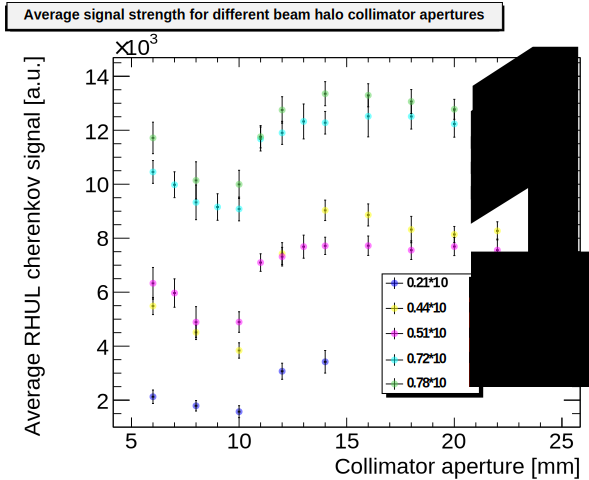
\includegraphics[width=\textwidth]{Figures/ATF/AverageSignal_perAperture.pdf}
\caption[RHUL Cherenkov detector signal vs. collimator aperture: different beam intensities]{Average signal as a function of the full aperture of the vertical beam halo collimator. The signal was measured for different beam intensities [\num{10e10}]: 0.21$\pm$0.02, 0.44$\pm$0.02, 0.51$\pm$0.02, 0.72$\pm$0.02 and 0.78$\pm$0.02, while the PMT voltage was constant at \SI{900}{\volt}. For each aperture, 500 ADC pulses were recorded, and the signal was averaged over the number of pulses. The error bars to the mean values are the standard deviation of the signal distributions at each point.\\For some scans, the data was not taken for all apertures. Therefore, especially the graph for the beam intensity of \num{0.21}$\pm$\num{0.02e10} is missing data points for the half millimetre steps and between 14 and \SI{24}{\milli\metre}.}
\label{fig:AverageSignal_Aperture_BeamIntensities}
\end{figure}
\begin{figure}
\centering
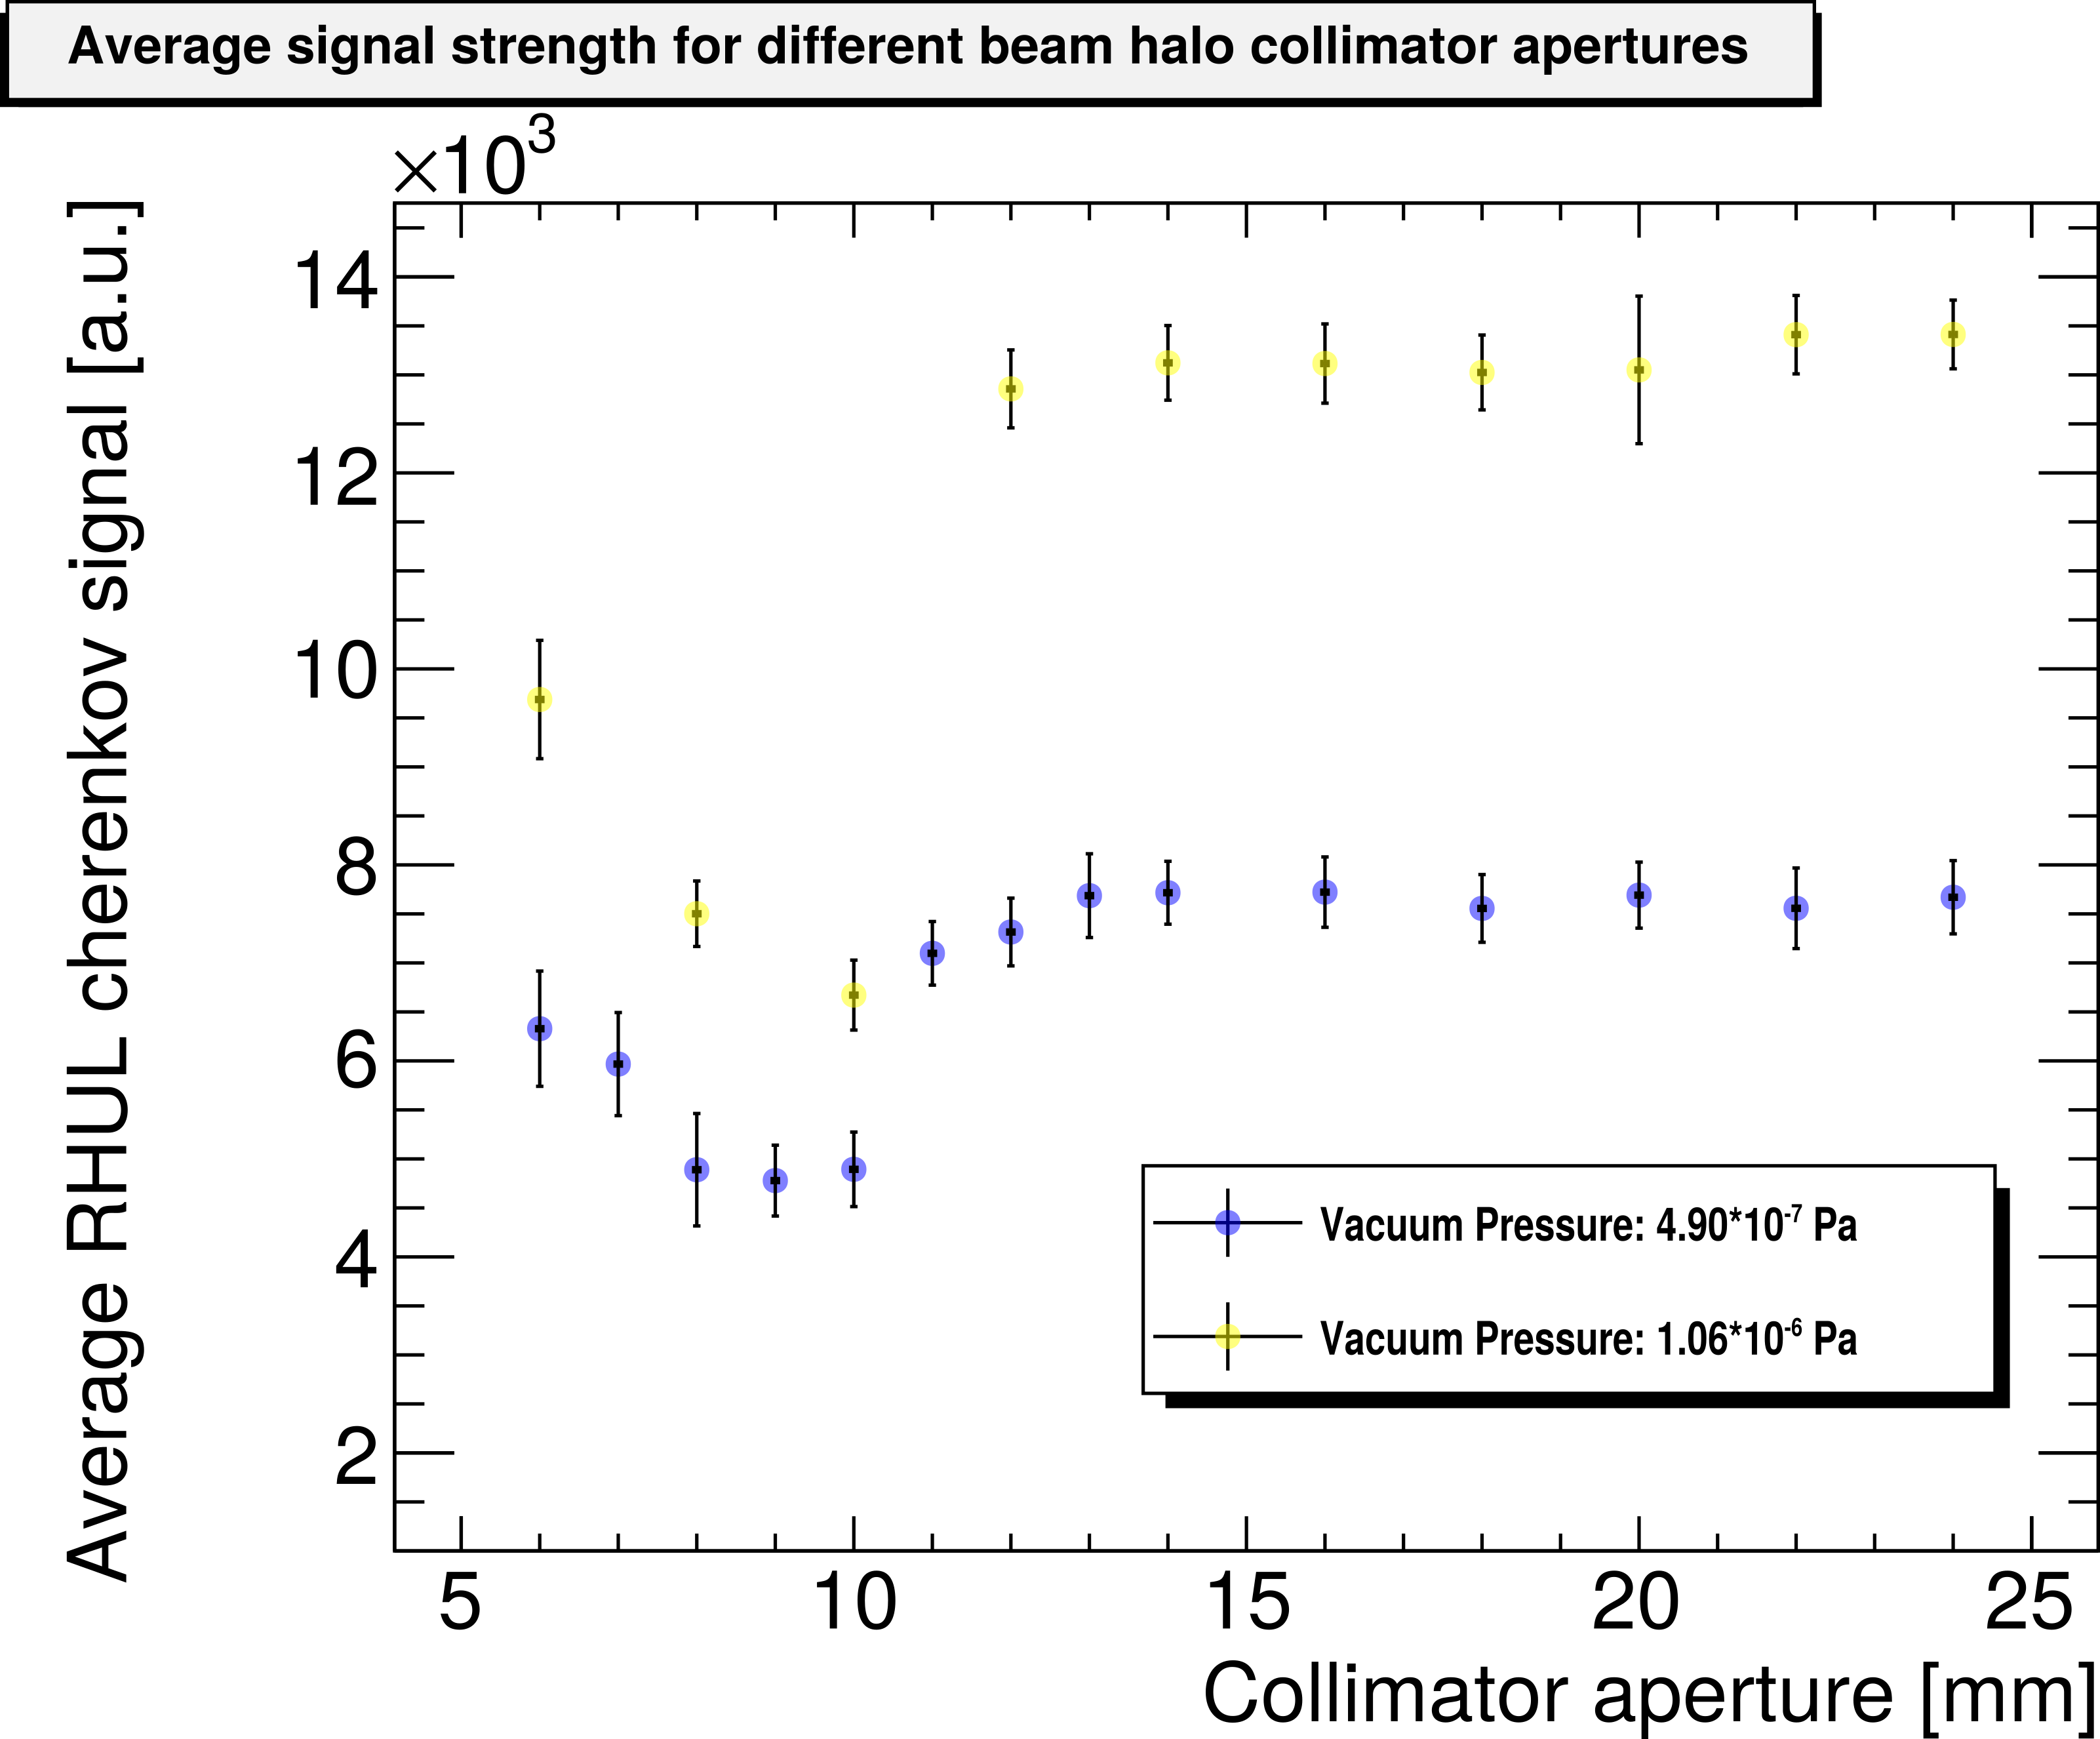
\includegraphics[width=\textwidth]{Figures/ATF/AverageSignal_perAperture_VacuumPressures.pdf}
\caption[RHUL Cherenkov detector signal vs. collimator aperture: different vacuum pressures]{Average signal as a function of the full aperture of the vertical beam halo collimator. The signal was measured for a beam intensity of \num{0.5}$\pm$\num{0.03e10} and a PMT voltage of \SI{900}{\volt}. The vacuum pressure was lowered from \SI{4.9e-7}{\pascal} to \SI{1.06e-6}{\pascal}. For each aperture, 500 ADC pulses were recorded, and the signal was averaged over the number of pulses. The error bars to the mean values are the standard deviation of the signal distributions at each point.}
\label{fig:AverageSignal_Aperture_VacuumPressures}
\end{figure}

\subsubsection{Test of the collimator alignment with respect to the beam position}
\label{collimator_alignment}
The next measurement sets are done to experimentally test whether the collimator is aligned in such a way that the beam is going through the centre between the jaws. The idea is that the background signal should be asymmetric if the beam is closer to one or the other side.\\Figure~\ref{fig:AverageSignal_HalfAperture} shows a plot of a measurement where one of the jaws was moved while the other jaw stayed in the fully extracted position. It is clear that moving the upper jaw shows the same characteristic background shape as before in the plots~\ref{fig:AverageSignal_Aperture_BeamIntensities} and \ref{fig:AverageSignal_Aperture_VacuumPressures}. But moving the lower jaw only shows no significant change in background. This leaves one with the possible conclusion that the beam is not in the centre between the two jaws but rather closer to the upper jaw. One could then say that also the background shape of the previous plots are only influenced by the upper jaw only. To confirm this conclusion, more measurements of this kind should be done to exclude a statistical fluctuation or simply a mistake in the process of data taking.
\newline
The next four figures show scans with asymmetric jaw positions around a certain value, i.e. 4 or \SI{5}{\milli\metre}. For each value, around which the jaws were moved, two measurements were done for the intensities of \num{0.84}$\pm$\num{0.03e10} and \num{1.01}$\pm$\num{0.03e10}. The plots are showing the background level in dependency of the position of the upper and lower jaw. As one jaw was moved in, the other one was simultaneously moved out, because of which the data line is diagonal in the diagrams. In all of the plots the drop in background level is clearly visible for a upper jaw position of \SI{5}{\milli\metre}, which follows the same behaviour as before. By closing the jaw more, the background level rises again and peaks for the minimal upper jaw position as the collimator jaw moves into the beam. All this seems to be consistent with the assumption that also here the lower jaw doesn't effect the beam in any way. Otherwise the plot would also show low background intensities for lower jaw positions of below \SI{5}{\milli\metre} which is not the case.\\
Especially significant is Figure~\ref{fig:AverageSignal_Asymmetric_5mm_101} with an identical background behaviour as in the measurements in Section~\ref{aperture_scans}. Also here it would be easier to make meaningful statements if the measurements would have more data points for larger jaw position regions, especially for the same positions in all plots.
\begin{figure}
\centering
\includegraphics[width=\textwidth]{Figures/ATF/AverageSignal_perJawPosition.pdf}
\caption[RHUL Cherenkov detector signal vs. collimator half aperture]{Average signal as a function of the position of the upper/lower jaw of the vertical beam halo collimator. The signal was measured for a beam intensity of \num{1.05}$\pm$\num{0.04e10} and a PMT voltage of \SI{800}{\volt}. First, the lower jaw was fixed to its open position (\SI{12}{\milli\metre}) and the upper jaw was moved to the positions plotted, then vice versa. For each jaw position, 500 ADC pulses were recorded, and the signal was averaged over the number of pulses. The error bars to the mean values are the standard deviation of the signal distributions at each point.}
\label{fig:AverageSignal_HalfAperture}
\end{figure}
\begin{figure}
\begin{subfigure}[b]{0.5\textwidth}
\includegraphics[width=\textwidth]{Figures/ATF/AsymmetricScan_4mm_beamintensity084_lego.pdf}
\end{subfigure}
\begin{subfigure}[b]{0.5\textwidth}
\includegraphics[width=\textwidth]{Figures/ATF/AsymmetricScan_4mm_beamintensity084_colz.pdf}
\end{subfigure}
\caption[RHUL Cherenkov detector signal for certain upper/lower jaw positions around \SI{4}{\milli\metre}, for a beam intensity of \num{0.84}$\pm$\num{0.03e10}]{Average signal as a function of the position of the upper and lower jaw of the vertical beam halo collimator. The signal was measured for a beam intensity of \num{0.84}$\pm$\num{0.03e10} and a PMT voltage of \SI{900}{\volt}. The jaws were moved simultaneously around \SI{4}{\milli\metre}. For each jaw position, at least 500 ADC pulses were recorded, and the signal was averaged over the number of pulses. The content of the bins were set to the appropriate average signal strength at that point.}
\label{fig:AverageSignal_Asymmetric_4mm_084}
\end{figure}
\begin{figure}
\begin{subfigure}[b]{0.5\textwidth}
\includegraphics[width=\textwidth]{Figures/ATF/AsymmetricScan_4mm_beamintensity101_lego.pdf}
\end{subfigure}
\begin{subfigure}[b]{0.5\textwidth}
\includegraphics[width=\textwidth]{Figures/ATF/AsymmetricScan_4mm_beamintensity101_colz.pdf}
\end{subfigure}
\caption[RHUL Cherenkov detector signal for certain upper/lower jaw positions around \SI{4}{\milli\metre}, for a beam intensity of \num{1.01}$\pm$\num{0.03e10}]{Average signal as a function of the position of the upper and lower jaw of the vertical beam halo collimator. The signal was measured for a beam intensity of \num{1.01}$\pm$\num{0.03e10} and a PMT voltage of \SI{900}{\volt}. The jaws were moved simultaneously around \SI{4}{\milli\metre}. For each jaw position, at least 500 ADC pulses were recorded, and the signal was averaged over the number of pulses. The content of the bins were set to the appropriate average signal strength at that point.}
\label{fig:AverageSignal_Asymmetric_4mm_101}
\end{figure}
\begin{figure}
\begin{subfigure}[b]{0.5\textwidth}
\includegraphics[width=\textwidth]{Figures/ATF/AsymmetricScan_5mm_beamintensity084_lego.pdf}
\end{subfigure}
\begin{subfigure}[b]{0.5\textwidth}
\includegraphics[width=\textwidth]{Figures/ATF/AsymmetricScan_5mm_beamintensity084_colz.pdf}
\end{subfigure}
\caption[RHUL Cherenkov detector signal for certain upper/lower jaw positions around \SI{5}{\milli\metre}, for a beam intensity of \num{0.84}$\pm$\num{0.03e10}]{Average signal as a function of the position of the upper and lower jaw of the vertical beam halo collimator. The signal was measured for a beam intensity of \num{0.84}$\pm$\num{0.03e10} and a PMT voltage of \SI{900}{\volt}. The jaws were moved simultaneously around \SI{5}{\milli\metre}. For each jaw position, at least 500 ADC pulses were recorded, and the signal was averaged over the number of pulses. The content of the bins were set to the appropriate average signal strength at that point.}
\label{fig:AverageSignal_Asymmetric_5mm_084}
\end{figure}
\begin{figure}
\begin{subfigure}[b]{0.5\textwidth}
\includegraphics[width=\textwidth]{Figures/ATF/AsymmetricScan_5mm_beamintensity101_lego.pdf}
\end{subfigure}
\begin{subfigure}[b]{0.5\textwidth}
\includegraphics[width=\textwidth]{Figures/ATF/AsymmetricScan_5mm_beamintensity101_colz.pdf}
\end{subfigure}
\caption[RHUL Cherenkov detector signal for certain upper/lower jaw positions around \SI{5}{\milli\metre}, for a beam intensity of \num{1.01}$\pm$\num{0.03e10}]{Average signal as a function of the position of the upper and lower jaw of the vertical beam halo collimator. The signal was measured for a beam intensity of \num{1.01}$\pm$\num{0.03e10} and a PMT voltage of \SI{900}{\volt}. The jaws were moved simultaneously around \SI{5}{\milli\metre}. For each jaw position, at least 500 ADC pulses were recorded, and the signal was averaged over the number of pulses. The content of the bins were set to the appropriate average signal strength at that point.}
\label{fig:AverageSignal_Asymmetric_5mm_101}
\end{figure}
%---------------------------------------------------
\subsection{Collimator as background source and attenuator}
\label{sec:BDSIM_sim}
As the data in the figures in the two previous sections have shown, the collimator reduces the existing background level if closed to an aperture of \SI{10}{\milli\metre}. By closing the jaws further, the background level increases again. The questions where this already existing background is coming from, and how the background is increased by the jaws driven into the beam, are now addresses by the following plots showing data from \bdsim simulations of the ATF2 lattice.

\begin{itemize}
 \item Number of particles at ATF2 line components - done, but has to be redone
 \item Number of particles at ATF2 IP - done, but has to be redone
\end{itemize}

\subsection{Effect on background level at IP}
\label{collimator_bkg_IP}
We have seen that the background level around the collimator area is dramatically affected by the movement of the collimator jaws. However, the actual effect of the collimator on the background level at the interaction point might be different, and is now discussed.

